% LayerTree: the talk.
%
% Build: make (pdflatex via latexmk). Diagrams are TikZ, drawn by the
% macros in ltmacros.tex; measured figures live in numbers.tex.
\documentclass[aspectratio=169,10pt]{beamer}
\usepackage{lmodern}
\usepackage[T1]{fontenc}
\usepackage[utf8]{inputenc}
\usepackage{xfp}
\usepackage{booktabs}
\usepackage{array}
\usepackage{tikz}
\usetikzlibrary{calc,arrows.meta,positioning,decorations.pathreplacing,shapes.misc,fit}
\usepackage{pgfplots}
\pgfplotsset{compat=1.18}
% LayerTree talk: colours, beamer theme and the tree-drawing macros.
%
% The palette is the explainer site's (site/css/tokens.css): cream paper,
% brown-black ink, one vermilion signal colour for the proof path.

\definecolor{ltbg}{HTML}{F4EDE0}
\definecolor{ltsurface}{HTML}{FBF7EF}
\definecolor{ltsurface2}{HTML}{EDE4D3}
\definecolor{ltink}{HTML}{2A2119}
\definecolor{ltmuted}{HTML}{5E5043}
\definecolor{ltborder}{HTML}{D9CDB8}
\definecolor{ltstrong}{HTML}{8A7B69}
\definecolor{ltaccent}{HTML}{D1481A}
\definecolor{ltaccentsoft}{HTML}{F8DDD0}
\definecolor{ltnode}{HTML}{2767AE}
\definecolor{ltnodesum}{HTML}{1E4E85}
\definecolor{ltleaf}{HTML}{1D8A6A}
\definecolor{ltexit}{HTML}{A67300}
\definecolor{ltchain}{HTML}{6B4E9B}
\definecolor{ltgood}{HTML}{2E7D32}
\definecolor{ltgoodsoft}{HTML}{DFECD6}
\definecolor{ltbad}{HTML}{A3201B}
\definecolor{ltbadsoft}{HTML}{F6D9D3}
\definecolor{ltempty}{HTML}{BCAE98}

% ---------------------------------------------------------------- theme
\setbeamercolor{background canvas}{bg=ltbg}
\setbeamercolor{normal text}{fg=ltink,bg=ltbg}
\setbeamercolor{frametitle}{fg=ltink,bg=ltbg}
\setbeamercolor{title}{fg=ltink}
\setbeamercolor{subtitle}{fg=ltmuted}
\setbeamercolor{structure}{fg=ltaccent}
\setbeamercolor{alerted text}{fg=ltaccent}
\setbeamercolor{block title}{fg=ltink,bg=ltsurface2}
\setbeamercolor{block body}{fg=ltink,bg=ltsurface}
\setbeamercolor{item}{fg=ltaccent}
\setbeamercolor{footline}{fg=ltmuted}
\setbeamerfont{frametitle}{size=\Large,series=\bfseries}
\setbeamerfont{title}{size=\huge,series=\bfseries}
\setbeamertemplate{navigation symbols}{}
\setbeamertemplate{itemize items}{\color{ltaccent}\raisebox{0.15ex}{\scriptsize$\blacksquare$}}
\setbeamertemplate{itemize subitem}{\color{ltstrong}\raisebox{0.2ex}{\tiny$\blacksquare$}}
\setbeamertemplate{blocks}[rounded][shadow=false]
\setbeamertemplate{frametitle}{%
  \vspace*{0.35cm}%
  \begin{beamercolorbox}[wd=\paperwidth,leftskip=0.6cm]{frametitle}%
    \usebeamerfont{frametitle}\insertframetitle%
    \ifx\insertframesubtitle\@empty\else\\[-0.1ex]{\normalsize\color{ltmuted}\mdseries\insertframesubtitle}\fi%
  \end{beamercolorbox}%
  \vspace*{-0.15cm}%
  {\color{ltaccent}\rule{1.4cm}{1.4pt}}\hspace*{-1.4cm}\hspace*{0.6cm}%
}
\setbeamertemplate{footline}{%
  \hbox to \paperwidth{\hspace*{0.6cm}{\tiny\color{ltmuted}\texttt{LayerTree}\quad\insertsectionhead}\hfill{\tiny\color{ltmuted}\insertframenumber}\hspace*{0.5cm}}\vspace*{0.25cm}}
\setbeamertemplate{section page}{%
  \vfill
  \begin{center}
    {\color{ltaccent}\rule{2cm}{2pt}}\\[0.6em]
    {\Huge\bfseries\insertsectionhead}\\[0.4em]
  \end{center}
  \vfill}
\AtBeginSection{\begin{frame}[plain]\sectionpage\end{frame}}

\newcommand{\code}[1]{{\ttfamily\small #1}}
\newcommand{\codes}[1]{{\ttfamily\scriptsize #1}}
\newcommand{\tr}[1]{\textsf{\textbf{#1}}}
\newcommand{\muted}[1]{{\color{ltmuted}#1}}
\newcommand{\hl}[1]{{\color{ltaccent}\textbf{#1}}}
\newcommand{\lnote}[1]{\par\vspace{0.3em}{\small\color{ltmuted}#1}}

% ---------------------------------------------------------- overlay keys
% Style keys that change with the overlay: visible on=<2->, alt=<2>{a}{b}.
\tikzset{
  invisible/.style={opacity=0,text opacity=0},
  visible on/.style={alt={#1{}{invisible}}},
  alt/.code args={<#1>#2#3}{\alt<#1>{\pgfkeysalso{#2}}{\pgfkeysalso{#3}}},
}

% ---------------------------------------------------------- tree styles
\tikzset{
  lt/edge/.style={draw=ltstrong,line width=0.6pt},
  lt/pathedge/.style={draw=ltaccent,line width=1.6pt},
  lt/inode/.style={circle,draw=ltnode,fill=ltsurface,line width=0.8pt,
    minimum size=0.62cm,inner sep=0pt,font=\scriptsize\bfseries,text=ltnodesum},
  lt/ianc/.style={lt/inode,draw=ltaccent,line width=1.4pt},
  lt/ifold/.style={lt/inode,draw=ltaccent,fill=ltaccent,text=white,line width=1.4pt},
  lt/isib/.style={lt/inode,draw=ltaccent,dashed,line width=1.2pt,fill=ltaccentsoft},
  lt/iempty/.style={lt/inode,draw=ltempty,text=ltempty,dashed},
  lt/root/.style={rectangle,rounded corners=2pt,draw=ltnode,fill=ltsurface,
    line width=0.9pt,minimum height=0.6cm,minimum width=1.3cm,inner sep=2pt,
    font=\scriptsize\bfseries,text=ltnodesum},
  lt/rootanc/.style={lt/root,draw=ltaccent,line width=1.4pt},
  lt/rootfold/.style={lt/root,fill=ltaccent,text=white,draw=ltaccent},
  lt/leafbase/.style={rectangle,rounded corners=2pt,line width=0.9pt,
    minimum width=1.12cm,minimum height=0.78cm,inner sep=1pt,align=center,
    font=\scriptsize},
  lt/leaf-n/.style={lt/leafbase,draw=ltleaf,fill=ltsurface},
  lt/leaf-e/.style={lt/leafbase,draw=ltempty,dashed,fill=ltbg,text=ltempty},
  lt/leaf-new/.style={lt/leafbase,draw=ltleaf,fill=ltgoodsoft,line width=1.4pt},
  lt/leaf-chg/.style={lt/leafbase,draw=ltaccent,fill=ltaccentsoft,line width=1.4pt},
  lt/leaf-out/.style={lt/leafbase,draw=ltexit,fill=ltexit!15,line width=1.4pt},
  lt/leaf-op/.style={lt/leafbase,draw=ltstrong,fill=ltsurface2},
  lt/leaf-pend/.style={lt/leafbase,draw=ltchain,fill=ltchain!12,line width=1.2pt},
  lt/leaf-land/.style={lt/leafbase,draw=ltnode,fill=ltnode!10,line width=1.2pt},
  lt/leaf-chan/.style={lt/leafbase,draw=ltleaf,fill=ltleaf!15,line width=1.2pt,double,double distance=0.6pt},
  lt/leaf-sib/.style={lt/leafbase,draw=ltaccent,dashed,fill=ltaccentsoft,line width=1.2pt},
  lt/region/.style={rounded corners=5pt,fill=ltnode!8,draw=ltnode!50,dashed,line width=0.6pt},
  lt/badge/.style={rectangle,rounded corners=2pt,inner sep=1.5pt,
    font=\tiny\bfseries,text=white},
  lt/badge-sig/.style={lt/badge,fill=ltleaf},
  lt/badge-op/.style={lt/badge,fill=ltstrong},
  lt/badge-hash/.style={lt/badge,fill=ltchain},
  lt/badge-voucher/.style={lt/badge,fill=ltnode},
  lt/badge-warn/.style={lt/badge,fill=ltbad},
  lt/badge-exit/.style={lt/badge,fill=ltexit},
  lt/chain/.style={rectangle,rounded corners=3pt,fill=ltchain,text=white,
    font=\scriptsize\bfseries,inner sep=4pt,align=center},
  lt/chainpend/.style={rectangle,rounded corners=3pt,draw=ltchain,dashed,
    line width=1pt,fill=ltsurface,text=ltchain,font=\scriptsize\bfseries,inner sep=4pt,align=center},
  lt/tx/.style={rectangle,rounded corners=3pt,draw=ltink,line width=0.8pt,
    fill=ltsurface,font=\scriptsize,align=left,inner sep=5pt,text width=3.6cm},
}

% Geometry: leaf i of a depth-3 tree sits at (i*\LTdx, 0); the node of
% height h and index j at the centre of its leaves, h*\LTdy up.
\newcommand{\LTdx}{1.38}
\newcommand{\LTdy}{1.05}
\newcommand{\LTx}[2]{\fpeval{(#2*2^(#1) + (2^(#1)-1)/2)*\LTdx}}

% \LTtree[keys]{a/5/n/note, b/3/n/, -/0/e/, ...}  (exactly 8 entries)
%   label/amount/style/note; style is one of n e new chg out op pend land chan sib.
% keys: path=p (the proof of position p: ancestors and siblings),
%       path2=q (a second proof), fold (ancestors filled: recomputed),
%       region=h/i (an aligned subtree highlighted), root text, out text,
%       pending (output drawn dashed: computed, not committed),
%       sibleaf (draw the leaf sibling of the path as a proof element).
\pgfkeys{/ltk/.is family,/ltk,
  path/.store in=\LTkpath, path=-1,
  path2/.store in=\LTkpathB, path2=-1,
  fold/.store in=\LTkfold, fold=0,
  region/.store in=\LTkregion, region={},
  regionlabel/.store in=\LTkregionlabel, regionlabel={},
  rootname/.store in=\LTkrootname, rootname={r},
  out/.store in=\LTkout, out={},
  pending/.store in=\LTkpending, pending=0,
  nosums/.store in=\LTknosums, nosums=0,
}

\makeatletter
\newcommand{\LTsetamt}[2]{\expandafter\xdef\csname lt@amt@#1\endcsname{#2}}
\newcommand{\LTamt}[1]{\csname lt@amt@#1\endcsname}
% Is node (h,j) an ancestor of position p? Sets \LTtmp to 1 or 0.
\newcommand{\LTisanc}[3]{% h j p
  \ifnum#3<0 \def\LTtmp{0}\else
  \edef\LTtmp{\fpeval{ (floor(#3/2^(#1)) == #2) ? 1 : 0 }}\fi}
\newcommand{\LTissib}[3]{% h j p
  \ifnum#3<0 \def\LTtmp{0}\else
  \edef\LTtmp{\fpeval{ ((floor(#3/2^(#1)) - 2*floor(floor(#3/2^(#1))/2) == 0 ?
      floor(#3/2^(#1))+1 : floor(#3/2^(#1))-1) == #2) ? 1 : 0 }}\fi}

\newcommand{\LTtree}[2][]{%
  \pgfkeys{/ltk,path=-1,path2=-1,fold=0,region={},regionlabel={},rootname={r},out={},pending=0,nosums=0,#1}%
  % Parse the leaves.
  \def\lt@i{0}%
  \foreach \lab/\amt/\sty/\nt [count=\ii from 0] in {#2} {%
    \LTsetamt{\ii}{\amt}%
    \expandafter\xdef\csname lt@lab@\ii\endcsname{\lab}%
    \expandafter\xdef\csname lt@sty@\ii\endcsname{\sty}%
    \expandafter\xdef\csname lt@nt@\ii\endcsname{\nt}%
  }%
  % Region background.
  \ifx\LTkregion\@empty\else
    \expandafter\lt@region\LTkregion\@nil
  \fi
  % Edges.
  \foreach \h in {1,2,3} {%
    \pgfmathtruncatemacro{\nj}{2^(3-\h)-1}%
    \foreach \j in {0,...,\nj} {%
      \foreach \c in {0,1} {%
        \pgfmathtruncatemacro{\ch}{\h-1}%
        \pgfmathtruncatemacro{\cj}{2*\j+\c}%
        \LTisanc{\ch}{\cj}{\LTkpath}\let\ea\LTtmp
        \LTisanc{\ch}{\cj}{\LTkpathB}\let\eb\LTtmp
        \ifnum\numexpr\ea+\eb\relax>0
          \draw[lt/pathedge] (\LTx{\h}{\j},\h*\LTdy) -- (\LTx{\ch}{\cj},\ch*\LTdy);
        \else
          \draw[lt/edge] (\LTx{\h}{\j},\h*\LTdy) -- (\LTx{\ch}{\cj},\ch*\LTdy);
        \fi
      }%
    }%
  }%
  % Sums of interior nodes.
  \foreach \j in {0,1,2,3} {%
    \pgfmathtruncatemacro{\a}{\LTamt{\the\numexpr2*\j\relax}+\LTamt{\the\numexpr2*\j+1\relax}}%
    \expandafter\xdef\csname lt@s@1@\j\endcsname{\a}}%
  \foreach \j in {0,1} {%
    \pgfmathtruncatemacro{\a}{\csname lt@s@1@\the\numexpr2*\j\relax\endcsname+\csname lt@s@1@\the\numexpr2*\j+1\relax\endcsname}%
    \expandafter\xdef\csname lt@s@2@\j\endcsname{\a}}%
  \pgfmathtruncatemacro{\a}{\csname lt@s@2@0\endcsname+\csname lt@s@2@1\endcsname}%
  \expandafter\xdef\csname lt@s@3@0\endcsname{\a}%
  % Interior nodes.
  \foreach \h in {1,2} {%
    \pgfmathtruncatemacro{\nj}{2^(3-\h)-1}%
    \foreach \j in {0,...,\nj} {%
      \def\st{lt/inode}%
      \edef\sm{\csname lt@s@\h @\j\endcsname}%
      \ifnum\sm=0 \def\st{lt/iempty}\fi
      \LTissib{\h}{\j}{\LTkpath}\ifnum\LTtmp=1 \def\st{lt/isib}\fi
      \LTissib{\h}{\j}{\LTkpathB}\ifnum\LTtmp=1 \def\st{lt/isib}\fi
      \LTisanc{\h}{\j}{\LTkpath}\ifnum\LTtmp=1 \ifnum\LTkfold=1 \def\st{lt/ifold}\else\def\st{lt/ianc}\fi\fi
      \LTisanc{\h}{\j}{\LTkpathB}\ifnum\LTtmp=1 \ifnum\LTkfold=1 \def\st{lt/ifold}\else\def\st{lt/ianc}\fi\fi
      \node[\st] (n-\h-\j) at (\LTx{\h}{\j},\h*\LTdy) {\ifnum\LTknosums=0 \sm\fi};
    }%
  }%
  % Root.
  \def\rst{lt/root}%
  \ifnum\LTkpath>-1 \ifnum\LTkfold=1 \def\rst{lt/rootfold}\else\def\rst{lt/rootanc}\fi\fi
  \node[\rst] (root) at (\LTx{3}{0},3*\LTdy) {\LTkrootname\ \ \csname lt@s@3@0\endcsname};
  % Leaves.
  \foreach \i in {0,...,7} {%
    \edef\sty{\csname lt@sty@\i\endcsname}%
    \LTissib{0}{\i}{\LTkpath}\let\sa\LTtmp
    \LTissib{0}{\i}{\LTkpathB}\let\sb\LTtmp
    \edef\full{\sty}%
    \ifnum\numexpr\sa+\sb\relax>0 \ifnum\pdfstrcmp{\sty}{e}=0 \else\edef\full{sib}\fi\fi
    \edef\lab{\csname lt@lab@\i\endcsname}%
    \edef\amt{\csname lt@amt@\i\endcsname}%
    \ifnum\pdfstrcmp{\sty}{e}=0
      \node[lt/leaf-e] (l-\i) at (\i*\LTdx,0) {$\varnothing$};
    \else
      \node[lt/leaf-\full] (l-\i) at (\i*\LTdx,0) {\textbf{\lab}\\[-1pt]\amt};
    \fi
    \edef\nt{\csname lt@nt@\i\endcsname}%
    \ifx\nt\@empty\else
      \node[font=\tiny,text=ltmuted,anchor=north,inner sep=1pt] at (l-\i.south) {\nt};
    \fi
  }%
  % The tree output on the chain.
  \ifx\LTkout\@empty\else
    \ifnum\LTkpending=1
      \node[lt/chainpend,anchor=south] (out) at (\LTx{3}{0},3*\LTdy+0.55) {\LTkout};
      \draw[ltchain,dashed,line width=0.8pt] (out.south) -- (root.north);
    \else
      \node[lt/chain,anchor=south] (out) at (\LTx{3}{0},3*\LTdy+0.55) {\LTkout};
      \draw[ltchain,line width=0.8pt] (out.south) -- (root.north);
    \fi
  \fi
}
\def\lt@region#1/#2\@nil{%
  \pgfmathsetmacro{\rx}{#2*2^(#1)*\LTdx-0.68}%
  \pgfmathsetmacro{\rX}{((#2+1)*2^(#1)-1)*\LTdx+0.68}%
  \pgfmathsetmacro{\rY}{#1*\LTdy+0.42}%
  \fill[lt/region] (\rx,-0.62) rectangle (\rX,\rY);
  \ifx\LTkregionlabel\@empty\else
    \node[font=\tiny\bfseries,text=ltnode,anchor=north west,inner sep=2pt] at (\rx,\rY) {\LTkregionlabel};
  \fi
}
\makeatother

% \LTbadge{pos}{text}{kind} under a leaf (row 1); \LTbadgeB for row 2.
\newcommand{\LTbadge}[3]{\node[lt/badge-#3,anchor=north] at ($(l-#1.south)+(0,-0.3)$) {#2};}
\newcommand{\LTbadgeB}[3]{\node[lt/badge-#3,anchor=north] at ($(l-#1.south)+(0,-0.62)$) {#2};}
% A badge on an interior node or the root.
\newcommand{\LTnbadge}[3]{\node[lt/badge-#3,anchor=south] at ($(#1.north)+(0,0.05)$) {#2};}

% Placeholder for an opcode (CCV + hypothetical Merkle-sum opcode) figure not yet measured.
\newcommand{\msuTBD}[1]{{\color{ltmuted}opcode: not yet measured}}

% Measured figures the slides quote, in one place so a re-measurement is
% one edit. Sources: spec/layertree.md 11, design/pending-receive.md,
% site/js/scaling.js, the suites' printed counts.
\newcommand{\nChecksFULL}{1,458}
\newcommand{\nChecksMID}{1,209}
\newcommand{\nChecksMIN}{57}
\newcommand{\nChecksCCV}{3,288}
\newcommand{\nChecksCHAN}{220}
\newcommand{\nChecksMSU}{126}
\newcommand{\nChecksTotal}{6,232}
\newcommand{\nLean}{72}
\newcommand{\nReplay}{387}
% Per active pending pair per window, R3 batch of 64 positions.
\newcommand{\nPairWindow}{587}
\newcommand{\nPairWindowFour}{1,006}
\newcommand{\nPairWindowSixteen}{664}
\newcommand{\nPairNoRthree}{1,105}

\newcommand{\chk}[2]{\item[{\alt<#1>{\color{ltgood}$\checkmark$}{\color{ltempty}$\circ$}}] #2}

\title{LayerTree}
\subtitle{One UTXO, an off-chain Merkle-sum tree,\\and a covenant that lets anyone leave in one transaction}
\author{Olaoluwa Osuntokun \texttt{(roasbeef)}}
\date{}

\begin{document}

% ======================================================================
\begin{frame}[plain]
  \begin{tikzpicture}[remember picture,overlay]
    \node[anchor=north west,inner sep=0] at ($(current page.north west)+(0.9,-1.2)$) {%
      \begin{minipage}{9.5cm}
        {\color{ltaccent}\rule{2cm}{2pt}}\\[0.8em]
        {\fontsize{34}{38}\selectfont\bfseries LayerTree}\\[0.8em]
        {\large\color{ltmuted} One UTXO, an off-chain Merkle-sum tree, and a covenant that lets anyone leave in one transaction}\\[2.2em]
        {\normalsize Olaoluwa Osuntokun \quad\texttt{roasbeef}}
      \end{minipage}};
    \begin{scope}[shift={($(current page.south east)+(-6.6,1.2)$)},scale=0.55,transform shape]
      \LTtree[out={tree output}]{A/5/n/, B/3/n/, C/6/n/, D/2/n/, E/4/n/, F/1/n/, -/0/e/, -/0/e/}
    \end{scope}
  \end{tikzpicture}
\end{frame}

% ======================================================================
\section{In five lines}

\begin{frame}{LayerTree in five lines}
  \begin{enumerate}
    \item One output commits to a Merkle-sum tree of balances; the tree is data, not transactions.
    \item Every transition proves an old node and folds a new one up the same path; the sums make theft structurally impossible.
    \item Anyone leaves in \hl{one transaction} with their own signature: 1,020 vB at 65,536 members from proposed opcodes (FULL); about 541 vB, plus 10 vB per doubling, with a hypothetical Merkle-sum opcode.
    \item Payments happen off-chain: channel leaves make it a Lightning sub-graph in one UTXO, vouchers and pending pairs give zero-byte receives.
    \item The cost is one queue for everyone, and opcodes that aren't active yet. Four tiers show exactly how few are needed.
  \end{enumerate}
  \vspace{1em}
  \centering
  {\small \texttt{layertree.tech} \quad \texttt{spec/layertree.md} \quad \texttt{paper/main.pdf}}
\end{frame}

% ======================================================================
\section{The problem}

\begin{frame}{Scaling is about ownership, not payments}
  \begin{itemize}
    \item Every distinct owner wants their own unspent output, and outputs are the scarce resource.
    \item So share one output between many owners. The hard part is not sharing, it's \hl{leaving}.
    \item Channel factories, CoinPool, Ark, timeout trees, CTV and CCV trees all answer the same way:
      the shared output is the root of a \hl{tree of transactions}.
    \item To leave alone you publish the path from the root to your leaf:
      $\log_2 N$ transactions, each with a fee and a confirmation, often against a deadline.
  \end{itemize}
  \vspace{0.6em}
  \begin{block}{}
    You pay for the sharing at exactly the moment you most need it to be cheap:
    when the operator is gone, fees are high and everyone else is leaving too.
  \end{block}
\end{frame}

\begin{frame}{Two shapes of shared output}
  \centering
  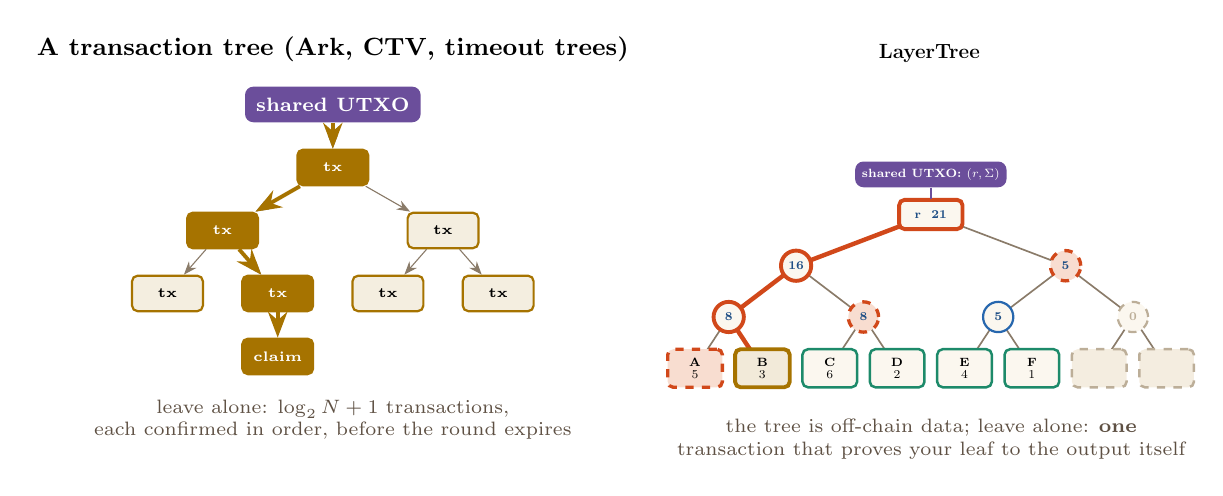
\begin{tikzpicture}[
      txn/.style={rectangle,rounded corners=2pt,draw=ltexit,fill=ltexit!12,line width=0.8pt,minimum width=0.9cm,minimum height=0.45cm,font=\tiny\bfseries},
      txp/.style={txn,fill=ltexit,text=white},
      >=Stealth]
    % Left: a transaction tree.
    \node[font=\small\bfseries] at (2.6,4.2) {A transaction tree (Ark, CTV, timeout trees)};
    \node[lt/chain] (u) at (2.6,3.5) {shared UTXO};
    \node[txp] (t0) at (2.6,2.7) {tx};
    \node[txp] (t1) at (1.2,1.9) {tx}; \node[txn] (t2) at (4.0,1.9) {tx};
    \node[txn] (t3) at (0.5,1.1) {tx}; \node[txp] (t4) at (1.9,1.1) {tx};
    \node[txn] (t5) at (3.3,1.1) {tx}; \node[txn] (t6) at (4.7,1.1) {tx};
    \foreach \a/\b in {u/t0,t0/t1,t0/t2,t1/t3,t1/t4,t2/t5,t2/t6} \draw[->,ltstrong] (\a) -- (\b);
    \foreach \a/\b in {u/t0,t0/t1,t1/t4} \draw[->,ltexit,line width=1.4pt] (\a) -- (\b);
    \node[txp] (cl) at (1.9,0.3) {claim};
    \draw[->,ltexit,line width=1.4pt] (t4) -- (cl);
    \node[align=center,font=\scriptsize,text=ltmuted] at (2.6,-0.5) {leave alone: $\log_2 N + 1$ transactions,\\each confirmed in order, before the round expires};
    % Right: LayerTree.
    \begin{scope}[shift={(7.2,0.15)},scale=0.62,transform shape]
      \node[font=\large\bfseries] at (4.8,6.45) {LayerTree};
      \LTtree[path=1,out={shared UTXO: $(r, \Sigma)$}]{A/5/n/, B/3/out/, C/6/n/, D/2/n/, E/4/n/, F/1/n/, -/0/e/, -/0/e/}
    \end{scope}
    \node[align=center,font=\scriptsize,text=ltmuted] at (10.2,-0.75) {the tree is off-chain data; leave alone: \textbf{one}\\transaction that proves your leaf to the output itself};
  \end{tikzpicture}
\end{frame}

\begin{frame}{The idea: the tree is data, and the output checks the proof}
  \begin{columns}[T]
    \begin{column}{0.52\textwidth}
      To leave, present your leaf and its Merkle proof \hl{to the output}. The spending script:
      \begin{enumerate}
        \item recomputes the root from your leaf and proof,
        \item checks it matches the root the output commits to,
        \item recomputes the root with your leaf removed,
        \item forces the transaction to recreate the shared output under that root and pay you.
      \end{enumerate}
      \vspace{0.4em}
      One transaction. No pre-signed tree. Nobody else's signature. No timelock.
    \end{column}
    \begin{column}{0.44\textwidth}
      \begin{block}{What it costs}
        About \textbf{32 vB per level} with proposed opcodes (FULL tier),
        \textbf{10 vB per doubling} with a hypothetical native Merkle-sum opcode.\\[0.4em]
        At 65,536 members: \textbf{1,020 vB} (FULL), \textbf{908 vB} (CCV),
        about \textbf{541 vB} (CCV + the hypothetical opcode).\\[0.4em]
        Constant in $N$ up to the depth: it does not grow with the number of members.
      \end{block}
    \end{column}
  \end{columns}
\end{frame}

% ======================================================================
\section{The construction}

\begin{frame}{A leaf is a 116-byte record}
  \centering
  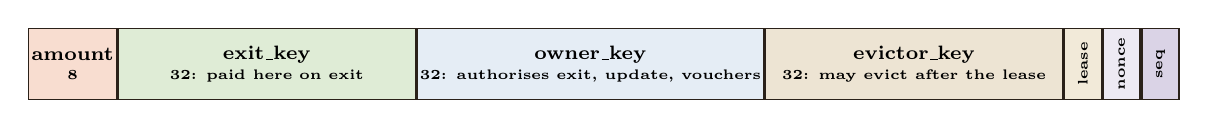
\begin{tikzpicture}[f/.style={rectangle,draw=ltink,line width=0.6pt,minimum height=0.9cm,font=\scriptsize\bfseries,align=center,inner sep=1pt}]
    \def\u{0.118}
    \node[f,fill=ltaccentsoft,minimum width=8*\u cm,anchor=west] (a) at (0,0) {amount\\[-1pt]\tiny 8};
    \node[f,fill=ltgoodsoft,minimum width=32*\u cm,anchor=west] (b) at (a.east) {exit\_key\\[-1pt]\tiny 32: paid here on exit};
    \node[f,fill=ltnode!12,minimum width=32*\u cm,anchor=west] (c) at (b.east) {owner\_key\\[-1pt]\tiny 32: authorises exit, update, vouchers};
    \node[f,fill=ltsurface2,minimum width=32*\u cm,anchor=west] (d) at (c.east) {evictor\_key\\[-1pt]\tiny 32: may evict after the lease};
    \node[f,fill=ltexit!15,minimum width=4*\u cm,anchor=west] (e) at (d.east) {\rotatebox{90}{\tiny lease}};
    \node[f,fill=ltchain!12,minimum width=4*\u cm,anchor=west] (g) at (e.east) {\rotatebox{90}{\tiny nonce}};
    \node[f,fill=ltchain!25,minimum width=4*\u cm,anchor=west] (h) at (g.east) {\rotatebox{90}{\tiny seq}};
  \end{tikzpicture}
  \vspace{1em}
  \begin{columns}[T]
    \begin{column}{0.48\textwidth}
      \begin{itemize}
        \item \code{exit\_key} $\neq$ \code{owner\_key}: a hot key authorises, a cold key (or a channel's funding key) receives.
        \item \code{evict\_after}: a \emph{lease}. Before it, nobody can remove you. After it, the evictor can, and only by paying you in full.
      \end{itemize}
    \end{column}
    \begin{column}{0.48\textwidth}
      \begin{itemize}
        \item \code{seq}: bumped by every carve, which is what makes vouchers single-use.
          \code{SEQ\_FINAL} marks a leaf whose amount is not the owner's alone (channel leaves).
        \item Node of a leaf: $(H_{\mathrm{leaf}}(\text{leaf}),\ \text{amount})$.
      \end{itemize}
    \end{column}
  \end{columns}
\end{frame}

\begin{frame}{A Merkle-\emph{sum} tree}
  \begin{columns}[c]
    \begin{column}{0.6\textwidth}
      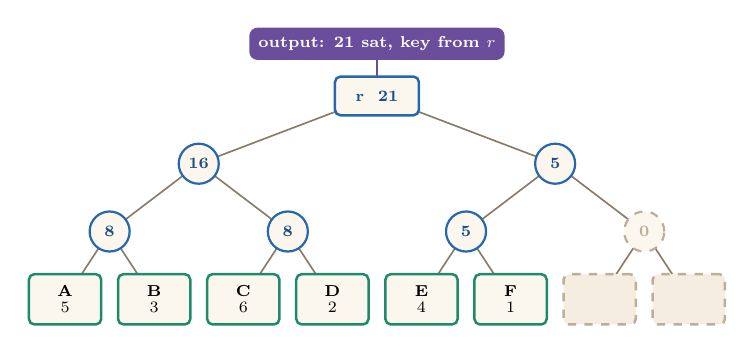
\begin{tikzpicture}[scale=0.82,transform shape]
        \LTtree[out={output: 21 sat, key from $r$}]{A/5/n/, B/3/n/, C/6/n/, D/2/n/, E/4/n/, F/1/n/, -/0/e/, -/0/e/}
      \end{tikzpicture}
    \end{column}
    \begin{column}{0.38\textwidth}
      \small
      Every node is a pair: a hash and an amount.
      {\footnotesize\[ \bigl(H_{\mathrm{node}}(l_h \| \mathrm{enc}(l_s) \| r_h \| \mathrm{enc}(r_s)),\ l_s + r_s\bigr) \]}
      The root commits to \emph{who} is in the tree and \emph{how much} they add up to,
      and the output's value must equal the root's sum.\\[0.6em]
      A script sees one leaf and one path, but because sums travel with hashes,
      verifying the path verifies the leaf's \hl{share of the total}.
      To steal you'd need a different tree with the same root.
    \end{column}
  \end{columns}
\end{frame}

\begin{frame}{State lives in the output's address}
  \centering
  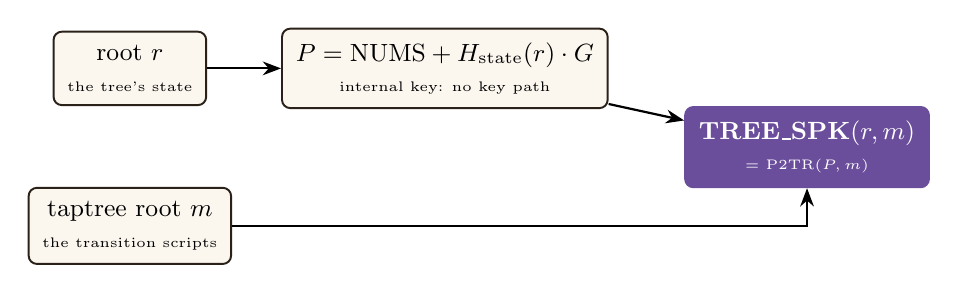
\begin{tikzpicture}[b/.style={rectangle,rounded corners=3pt,draw=ltink,fill=ltsurface,line width=0.7pt,font=\small,align=center,inner sep=5pt},>=Stealth]
    \node[b] (r) at (0,2) {root $r$\\\tiny the tree's state};
    \node[b] (P) at (4,2) {$P = \mathrm{NUMS} + H_{\mathrm{state}}(r)\cdot G$\\\tiny internal key: no key path};
    \node[b] (m) at (0,0) {taptree root $m$\\\tiny the transition scripts};
    \node[b,fill=ltchain,text=white,draw=ltchain] (o) at (8.6,1) {\textbf{TREE\_SPK$(r, m)$}\\\tiny = P2TR$(P, m)$};
    \draw[->,thick] (r) -- (P);
    \draw[->,thick] (P) -- (o);
    \draw[->,thick] (m) -| ($(o.south)+(0,0)$);
  \end{tikzpicture}
  \vspace{0.6em}
  \begin{itemize}
    \item Change one balance and the address changes. The output \emph{is} the state machine.
    \item Scripts get the claimed $r$ and $m$ in the witness, recompute the output key, and compare it with the coin being spent (and the one being created). Lie about the root and the keys don't match.
    \item $m$ binds the rule set too: you can't recreate the output under rules of your own choosing.
    \item Under CCV (BIP-443) the same binding is the data tweak \code{sha256(NUMS || r)}, checked natively by \code{OP\_CHECKCONTRACTVERIFY}.
  \end{itemize}
\end{frame}

\begin{frame}{Every transition is the same machine}
  \begin{columns}[T]
    \begin{column}{0.44\textwidth}
      A \hl{step}: prove an old node against the current root, then fold a new node up the \emph{same} siblings to get the next root.
      \begin{itemize}
        \item exit: leaf $\to$ empty
        \item join: empty $\to$ leaf or subtree
        \item update: leaf $\to$ leaf
        \item carve: two steps, shrink one leaf, fill an empty slot
      \end{itemize}
      Tapscript has no loops, so every batch size is a different script: a different tapleaf in the taptree, chosen at creation.
    \end{column}
    \begin{column}{0.54\textwidth}
      \scriptsize
      \begin{tabular}{@{}lll@{}}
        \toprule
        Transition & Who & Does \\ \midrule
        \tr{EXIT} & owner & leaf $\to\varnothing$, pay exit key \\
        \tr{JOIN} & operator & $\varnothing\to$ leaf / cohort \\
        \tr{UPDATE} & owner + op & rewrite a leaf \\
        \tr{EVICT} & evictor, after lease & exit, paid in full \\
        \tr{CLAIM} & voucher holder & carve a new leaf \\
        \tr{SPLIT} & owner & carve, signed directly \\
        \tr{REWRITE}$_h$ & changed owners + op & a cohort at once \\
        \tr{DETACH}$_h$ & operator & cohort to own output \\
        \tr{RECLAIM} & op, after deadline & pending leaf back \\
        \bottomrule
      \end{tabular}
    \end{column}
  \end{columns}
\end{frame}

\begin{frame}{The covenant makes three checks}
  \begin{columns}[c]
    \begin{column}{0.62\textwidth}
      \begin{tikzpicture}[scale=0.8,transform shape]
        \only<1>{\LTtree[out={tree output, 21}]{A/5/n/, B/3/n/, C/6/n/, D/2/n/, E/4/n/, F/1/n/, -/0/e/, -/0/e/}}
        \only<2>{\LTtree[path=1,out={tree output, 21}]{A/5/n/, B/3/out/, C/6/n/, D/2/n/, E/4/n/, F/1/n/, -/0/e/, -/0/e/}\LTbadge{1}{B signs}{sig}}
        \only<3>{\LTtree[path=1,out={tree output, 21}]{A/5/n/, B/3/out/, C/6/n/, D/2/n/, E/4/n/, F/1/n/, -/0/e/, -/0/e/}\LTbadge{1}{B signs}{sig}}
        \only<4->{\LTtree[path=1,fold=1,rootname={r'},out={new output, 18}]{A/5/n/, -/0/e/, C/6/n/, D/2/n/, E/4/n/, F/1/n/, -/0/e/, -/0/e/}\LTbadge{1}{paid 3}{exit}}
      \end{tikzpicture}
    \end{column}
    \begin{column}{0.36\textwidth}
      \small
      \begin{itemize}
        \chk{2-}{\textbf{The input commits to the old root.} Fold B's leaf with its three siblings; derive the key; compare.}
        \chk{3-}{\textbf{The rule holds.} B signed; B's payout is exactly 3 to B's exit key.}
        \chk{4-}{\textbf{The output commits to the new root.} Fold $\varnothing$ up the same siblings; output 0 must be TREE\_SPK$(r')$ with 18.}
      \end{itemize}
      \vspace{0.5em}
      \only<1>{\muted{The chain holds a commitment and an amount. Everything else lives off-chain with the members.}}
      \only<2>{\muted{Witness: B's leaf, a sibling per level, $r$, $m$, B's signature.}}
      \only<3>{\muted{The rule is the only part that differs between transitions.}}
      \only<4>{\muted{Same siblings, folded twice. That's the whole cost, and it depends on depth, not membership.}}
    \end{column}
  \end{columns}
\end{frame}

% ======================================================================
\section{The transitions, step by step}

\begin{frame}{EXIT: leaving needs only your own signature}
  \begin{columns}[c]
    \begin{column}{0.66\textwidth}
      \begin{tikzpicture}[scale=0.85,transform shape]
        \only<1>{\LTtree[out={tree output, 21}]{A/5/n/, B/3/n/, C/6/out/, D/2/n/, E/4/n/, F/1/n/, -/0/e/, -/0/e/}\LTbadge{2}{C signs}{sig}}
        \only<2>{\LTtree[path=2,out={tree output, 21}]{A/5/n/, B/3/n/, C/6/out/, D/2/n/, E/4/n/, F/1/n/, -/0/e/, -/0/e/}\LTbadge{2}{C signs}{sig}}
        \only<3>{\LTtree[path=2,fold=1,rootname={r'},out={computed: 15},pending=1]{A/5/n/, B/3/n/, -/0/e/, D/2/n/, E/4/n/, F/1/n/, -/0/e/, -/0/e/}}
        \only<4->{\LTtree[path=2,fold=1,rootname={r'},out={new output, 15}]{A/5/n/, B/3/n/, -/0/e/, D/2/n/, E/4/n/, F/1/n/, -/0/e/, -/0/e/}\LTbadge{2}{paid 6}{exit}}
      \end{tikzpicture}
    \end{column}
    \begin{column}{0.32\textwidth}
      \small
      \only<1>{C decides to leave. No permission, no counterparty, no pre-signed transaction: C builds a transaction spending the tree output and signs it with the owner key.}
      \only<2>{The witness carries C's leaf and three siblings: D, the node over A and B, the node over the right half. Folding gives $8 \to 16 \to 21$: the committed root.}
      \only<3>{Fold again with $\varnothing$ in C's place, same siblings: $2 \to 10 \to 15$.}
      \only<4>{Output 0 recreates the tree with exactly 15; output 1 pays C's exit key 6.\\[0.5em]
        \textbf{Depth 16: 1,020 vB (FULL), 908 (CCV), about 520 (CCV + hypothetical Merkle-sum opcode, MSU).}\\[0.2em]\muted{\scriptsize MSU: full dense depth-16 tree; 541 at $2^{16}$ members, key-addressed.}\\[0.3em]
        \muted{Exact-payout trees (\tr{EXIT}$^=$) pay fees from a separate input, so nobody can shave a payout.}}
      \only<5>{\textbf{\tr{EXIT}$_K^t$}: the owner signs once, off-chain, over $H_{\mathrm{exit}}(\text{tree\_id}\,\|\,\text{body(leaf)})$.
        A tower builds and rebuilds the exit with the owner offline.
        It survives top-ups, and pays only the owner's exit key: a bearer right to \emph{when}, never \emph{where}.}
    \end{column}
  \end{columns}
\end{frame}

\begin{frame}{JOIN: one member, or a whole cohort for one price}
  \begin{columns}[c]
    \begin{column}{0.66\textwidth}
      \begin{tikzpicture}[scale=0.85,transform shape]
        \only<1>{\LTtree[path=2,out={tree output, 9}]{Op/4/op/, A/5/n/, -/0/e/, -/0/e/, -/0/e/, -/0/e/, -/0/e/, -/0/e/}\LTbadge{2}{operator signs}{op}}
        \only<2>{\LTtree[path=2,fold=1,rootname={r'},out={tree output, 11}]{Op/4/op/, A/5/n/, E/2/new/, -/0/e/, -/0/e/, -/0/e/, -/0/e/, -/0/e/}\LTbadge{2}{funded: +2}{sig}}
        \only<3>{\LTtree[region=2/1,regionlabel={cohort, built off-chain},out={tree output, 11}]{Op/4/op/, A/5/n/, E/2/n/, -/0/e/, F/3/new/, G/5/new/, H/6/new/, J/2/new/}}
        \only<4->{\LTtree[region=2/1,regionlabel={grafted: one node},rootname={r'},out={tree output, 27}]{Op/4/op/, A/5/n/, E/2/n/, -/0/e/, F/3/n/, G/5/n/, H/6/n/, J/2/n/}\LTnbadge{n-2-1}{proves $E_2$ empty}{op}}
      \end{tikzpicture}
    \end{column}
    \begin{column}{0.32\textwidth}
      \small
      \only<1>{Only the operator adds leaves. A single join proves that a slot holds the empty node, with the same kind of proof an exit uses.}
      \only<2>{E's leaf folds up the same path. The output must grow by exactly 2, brought in by another input. \textbf{Single \tr{JOIN}$_0$, depth 16: 937 vB (FULL).} Hypothetical Merkle-sum opcode (MSU): script 237 B and 225 B of witness, \muted{vB not stated in the note.}}
      \only<3>{For a cohort the operator builds a subtree off-chain and sends each joiner their leaf and path. \hl{Each joiner checks their own path before paying.}}
      \only<4>{The graft proves one empty node of height 2 and replaces it with the cohort's node. The covenant never looks inside.\\[0.4em]
        \textbf{256 members: 679 vB. 1,024: 614 vB} (FULL, cohort \tr{JOIN}$_h$; \msuTBD{join-h}). Under 1 vB per member, against 43 vB for an output in a batch.\\[0.3em]
        \muted{A bad graft freezes value, it can't create or steal any: the sums still balance.}}
    \end{column}
  \end{columns}
\end{frame}

\begin{frame}{UPDATE, and the top-up that needs no owner}
  \begin{columns}[c]
    \begin{column}{0.66\textwidth}
      \begin{tikzpicture}[scale=0.85,transform shape]
        \only<1>{\LTtree[path=4,out={tree output, 21}]{A/5/n/, B/3/n/, C/6/n/, D/2/n/, E/4/chg/lease 900, F/1/n/, -/0/e/, -/0/e/}\LTbadge{4}{E signs}{sig}\LTbadgeB{4}{operator signs}{op}}
        \only<2>{\LTtree[path=4,fold=1,rootname={r'},out={tree output, 21}]{A/5/n/, B/3/n/, C/6/n/, D/2/n/, E/4/new/lease 1900, F/1/n/, -/0/e/, -/0/e/}}
        \only<3->{\LTtree[path=4,fold=1,rootname={r''},out={tree output, 24}]{A/5/n/, B/3/n/, C/6/n/, D/2/n/, E/7/new/lease 1900, F/1/n/, -/0/e/, -/0/e/}\LTbadge{4}{only operator}{op}}
      \end{tikzpicture}
    \end{column}
    \begin{column}{0.32\textwidth}
      \small
      \only<1>{\tr{UPDATE} rewrites a leaf in place: resize, renew the lease, rotate keys. It needs the owner \emph{and} the operator.}
      \only<2>{Here E renews its lease. One step, about 1,030 vB alone (FULL; \msuTBD{update}), which is why payments must not do this one at a time.}
      \only<3>{An \hl{amount-only increase} needs no owner signature: nobody can use it to rotate a key or shorten a lease. The operator tops E up by 3 from its own funds.\\[0.4em]
        \muted{Except on a \code{SEQ\_FINAL} leaf: a channel leaf's amount is the capacity its signed states commit to, so changing it needs the owner.}}
    \end{column}
  \end{columns}
\end{frame}

\begin{frame}{Leases, eviction and the cohort sweep}
  \begin{columns}[c]
    \begin{column}{0.66\textwidth}
      \begin{tikzpicture}[scale=0.85,transform shape]
        \only<1>{\LTtree[region=2/1,regionlabel={cohort, lease 900},out={tree output, 25}]{Op/4/op/, X/3/n/no lease, Y/2/n/lease 500, -/0/e/, A/5/n/, B/3/n/, C/6/n/, D/2/n/}}
        \only<2>{\LTtree[path=2,region=2/1,regionlabel={cohort, lease 900},out={tree output, 25}]{Op/4/op/, X/3/n/no lease, Y/2/out/lease 500, -/0/e/, A/5/n/, B/3/n/, C/6/n/, D/2/n/}\LTbadgeB{2}{op signs, locktime $\geq$ 500}{op}}
        \only<3>{\LTtree[path=2,fold=1,rootname={r'},region=2/1,regionlabel={cohort, lease 900},out={tree output, 23}]{Op/4/op/, X/3/n/no lease, -/0/e/, -/0/e/, A/5/n/, B/3/n/, C/6/n/, D/2/n/}\LTbadge{2}{paid 2}{exit}}
        \only<4->{\LTtree[region=2/1,regionlabel={swept at height 900},rootname={r''},out={tree output, 7}]{Op/4/op/, X/3/n/no lease, -/0/e/, -/0/e/, -/0/e/, -/0/e/, -/0/e/, -/0/e/}\LTbadge{4}{5}{exit}\LTbadge{5}{3}{exit}\LTbadge{6}{6}{exit}\LTbadge{7}{2}{exit}}
      \end{tikzpicture}
    \end{column}
    \begin{column}{0.32\textwidth}
      \small
      \only<1>{Every leaf names an evictor and a lease height. X's evictor is NUMS: X can never be evicted.}
      \only<2>{An eviction is an exit signed by the evictor, in a transaction whose \code{nLockTime} is at least the lease.}
      \only<3>{The payout must equal Y's amount exactly. The operator can remove Y but cannot take a satoshi of it.}
      \only<4>{\tr{EVICT\_SUBTREE}$_h$ publishes the cohort's slots once, checks every lease, pays every leaf, and proves one path.\\[0.4em]
        \textbf{13 leaves: 203 vB each. 51 leaves: 158 vB each} (FULL; \msuTBD{sweep}).\\[0.3em]
        \muted{Cheap eviction cuts both ways: it reclaims dead weight and it makes griefing cheap. Members who want a hard guarantee hold a long lease.}}
    \end{column}
  \end{columns}
\end{frame}

\begin{frame}{Vouchers: CLAIM carves a new leaf out of yours}
  \begin{columns}[c]
    \begin{column}{0.66\textwidth}
      \begin{tikzpicture}[scale=0.85,transform shape]
        \only<1>{\LTtree[out={tree output, 29}]{A/8/n/seq 0, B/3/n/, C/6/n/, D/2/n/, -/0/e/, -/0/e/, -/0/e/, Q/10/n/}\LTbadgeB{0}{voucher: 3 to V}{voucher}}
        \only<2>{\LTtree[path=0,fold=1,rootname={r$_{1/2}$},out={intermediate},pending=1]{A/5/chg/seq 1, B/3/n/, C/6/n/, D/2/n/, -/0/e/, -/0/e/, -/0/e/, Q/10/n/}\LTbadgeB{0}{A's signature checked}{voucher}}
        \only<3->{\LTtree[path=4,fold=1,rootname={r'},out={tree output, 29}]{A/5/n/seq 1, B/3/n/, C/6/n/, D/2/n/, V/3/new/, -/0/e/, -/0/e/, Q/10/n/}}
      \end{tikzpicture}
    \end{column}
    \begin{column}{0.32\textwidth}
      \small
      \only<1>{A signs a message naming its own leaf (without the amount), \code{tree\_id}, and a new leaf giving 3 to V. Nothing happens on-chain.}
      \only<2>{V's \tr{CLAIM} proves A's leaf and checks A's signature with \code{OP\_CHECKSIGFROMSTACK}. A's leaf shrinks by 3 and its \code{seq} goes up.}
      \only<3>{A second proof, under the intermediate root, shows slot 4 is empty, and V's leaf goes there. Total unchanged.\\[0.4em]
        \hl{Single use for free:} the message binds A's \code{seq}, so it never verifies again.\\[0.3em]
        \muted{The covenant stops over-redemption, not over-issuance: an unredeemed voucher is credit.}}
    \end{column}
  \end{columns}
\end{frame}

\begin{frame}{The voucher family}
  \small
  \begin{tabular}{@{}p{2.0cm}>{\raggedright\arraybackslash}p{6.2cm}>{\raggedright\arraybackslash}p{5.8cm}@{}}
    \toprule
    Form & What it adds & What it's for \\ \midrule
    \tr{CLAIM} & owner's signature over the carve & pay someone not yet in the tree \\
    \tr{SPLIT} & signature over the transaction instead & the same carve without CSFS: exists in MIN \\
    \tr{CLAIM}$^h$ & a 32-byte preimage hashed \emph{into} the signed message & an HTLC: atomic swaps against Lightning \\
    \tr{CLAIM}$^x$, $^{hx}$ & a signature by the source's \emph{exit} key too & a credit leaf the operator can't drain \\
    \tr{CLAIM}$^m$, $^{hm}$ & target is the sibling, raised to an absolute amount & the atomic receive; tower-redeemable \\
    \bottomrule
  \end{tabular}
  \vspace{0.8em}
  \begin{itemize}
    \item The hash lock costs 8 bytes and no opcode: a wrong preimage just produces an invalid signature.
    \item A voucher can have no on-chain deadline: script can say ``not before'', never ``not after''. Deadlines live in the other leg of a swap, or in the source leaf itself (the pending leaf, later).
    \item Vouchers bind \code{tree\_id}, unique per lineage, so they can't be replayed against a sibling tree with the same rules.
  \end{itemize}
\end{frame}

\begin{frame}{Swaps: a voucher and an HTLC on one secret}
  \centering
  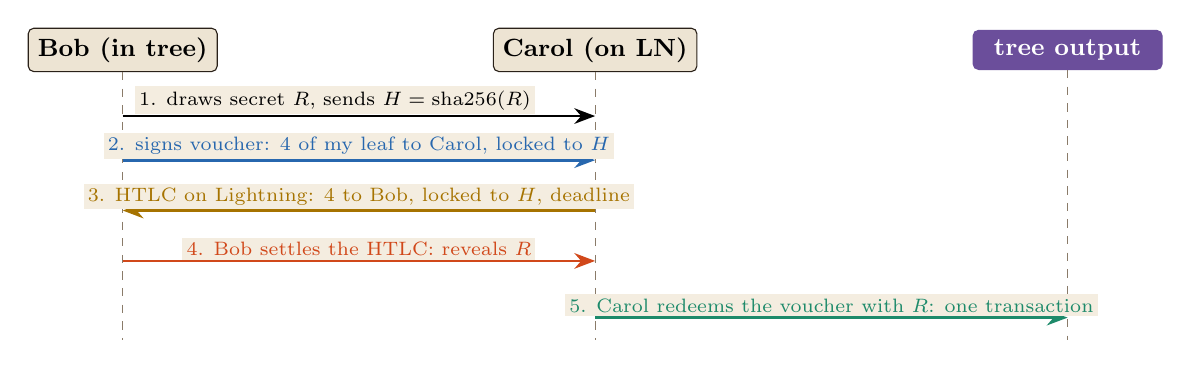
\begin{tikzpicture}[y=0.8cm,>=Stealth,lane/.style={draw=ltstrong,dashed},
      who/.style={rectangle,rounded corners=2pt,fill=ltsurface2,draw=ltink,font=\small\bfseries,minimum width=2.4cm},
      msg/.style={->,line width=1pt},lab/.style={font=\scriptsize,fill=ltbg,inner sep=1.5pt}]
    \node[who] (b) at (0,0) {Bob (in tree)};
    \node[who] (c) at (6,0) {Carol (on LN)};
    \node[who,fill=ltchain,text=white,draw=ltchain] (t) at (12,0) {tree output};
    \draw[lane] (b) -- (0,-4.6); \draw[lane] (c) -- (6,-4.6); \draw[lane] (t) -- (12,-4.6);
    \uncover<1->{\node[lab,anchor=west] at (0.15,-0.8) {1. draws secret $R$, sends $H = \mathrm{sha256}(R)$};
      \draw[msg] (0,-1.05) -- (6,-1.05);}
    \uncover<2->{\draw[msg,ltnode] (0,-1.75) -- node[lab,above] {2. signs voucher: 4 of my leaf to Carol, locked to $H$} (6,-1.75);}
    \uncover<3->{\draw[msg,ltexit] (6,-2.55) -- node[lab,above] {3. HTLC on Lightning: 4 to Bob, locked to $H$, deadline} (0,-2.55);}
    \uncover<4->{\draw[msg,ltaccent] (0,-3.35) -- node[lab,above] {4. Bob settles the HTLC: reveals $R$} (6,-3.35);}
    \uncover<5->{\draw[msg,ltleaf] (6,-4.25) -- node[lab,above] {5. Carol redeems the voucher with $R$: one transaction} (12,-4.25);}
  \end{tikzpicture}
  \vspace{-0.2em}
  \begin{itemize}\footnotesize
    \item<5-> The HTLC has a deadline and the voucher doesn't, which fixes the order: the secret comes from the party the HTLC pays, and the deadline-free leg resolves \emph{second}.
    \item<5-> Done right, the Lightning leg settles off-chain and the whole swap is one transaction. Buy a leaf with Lightning sats while holding no on-chain bitcoin at all.
  \end{itemize}
\end{frame}

\begin{frame}{REWRITE$_h$: a cohort in one transaction}
  \begin{columns}[c]
    \begin{column}{0.66\textwidth}
      \begin{tikzpicture}[scale=0.85,transform shape]
        \only<1>{\LTtree[path=1,region=2/1,regionlabel={cohort},out={tree output, 21}]{Op/4/op/, Q/3/n/, -/0/e/, -/0/e/, A/5/n/, B/3/n/, C/6/n/, -/0/e/}\LTnbadge{n-2-1}{one shared path}{op}}
        \only<2>{\LTtree[region=2/1,regionlabel={old and new published},out={tree output, 21}]{Op/4/op/, Q/3/n/, -/0/e/, -/0/e/, -/0/out/, B/2/chg/, C/7/chg/, N/4/new/}\LTbadge{4}{A signs}{sig}\LTbadge{5}{B signs}{sig}\LTbadge{6}{no sig}{voucher}\LTbadge{7}{funded}{sig}}
        \only<3->{\LTtree[path=1,fold=1,rootname={r'},region=2/1,regionlabel={rewritten},out={tree output, 20}]{Op/4/op/, Q/3/n/, -/0/e/, -/0/e/, -/0/e/, B/2/n/, C/7/n/, N/4/n/}\LTbadge{4}{A paid 5}{exit}}
      \end{tikzpicture}
    \end{column}
    \begin{column}{0.32\textwidth}
      \small
      \only<1>{A, B and C were grafted together, so above their subtree they share one path.}
      \only<2>{In one rewrite: A leaves, B pays C 1, N joins. The witness has every slot twice, before and after. A and B sign because their leaves change. C's change is amount-only, so C needn't sign. The operator signs once.}
      \only<3>{The script rebuilds the old subtree, checks it against the root, rebuilds the new one and folds it up the same path. A is paid exactly 5; N's 4 comes from an input.\\[0.4em]
        \textbf{64 positions: 151 vB per changed leaf (vs 1,030 per \tr{UPDATE}), 165 per exit, 95 per leaf left alone} (a one-byte ``unchanged'' marker). All FULL; \msuTBD{rewrite-mixed}.}
    \end{column}
  \end{columns}
\end{frame}

\begin{frame}{DETACH$_h$: a cohort gets its own output}
  \begin{columns}[c]
    \begin{column}{0.6\textwidth}
      \begin{tikzpicture}[scale=0.8,transform shape]
        \only<1>{\LTtree[path=4,region=2/1,regionlabel={cohort},out={tree output, 23}]{Op/4/op/, Q/3/n/, -/0/e/, -/0/e/, -/0/e/, B/2/n/, C/7/n/, N/4/n/}\LTnbadge{n-2-1}{operator signs}{op}}
        \only<2->{\LTtree[nosums=0,out={parent output, 7}]{Op/4/op/, Q/3/n/, -/0/e/, -/0/e/, -/0/e/, -/0/e/, -/0/e/, -/0/e/}
          \node[lt/chain] at (8.3,4.6) {child output, 13};
          \draw[ltchain,line width=0.8pt] (8.3,4.3) -- (8.3,2.6);
          \node[font=\scriptsize,text=ltnode,align=left,anchor=west] at (8.45,3.4) {the cohort's\\subtree, now\\its own root};}
      \end{tikzpicture}
    \end{column}
    \begin{column}{0.38\textwidth}
      \small
      The operator moves an aligned subtree into a tree output of its own, under the same option set and \code{tree\_id}.\\[0.5em]
      \uncover<2->{The cohort's node becomes the root of a depth-$h$ tree. Members' proofs still work: they just stop $D-h$ levels early.
      \begin{itemize}
        \item later exits pay $h$ levels, not $D$
        \item the cohort gets its own mempool chain
        \item about 780 vB (FULL), 621 under CCV; \msuTBD{detach}
      \end{itemize}
      It's the structural answer to contention: shard on demand.}
    \end{column}
  \end{columns}
\end{frame}

% ======================================================================
\section{Lightning}

\begin{frame}{Channel leaves: a Lightning sub-graph in one UTXO}
  \begin{columns}[c]
    \begin{column}{0.58\textwidth}
      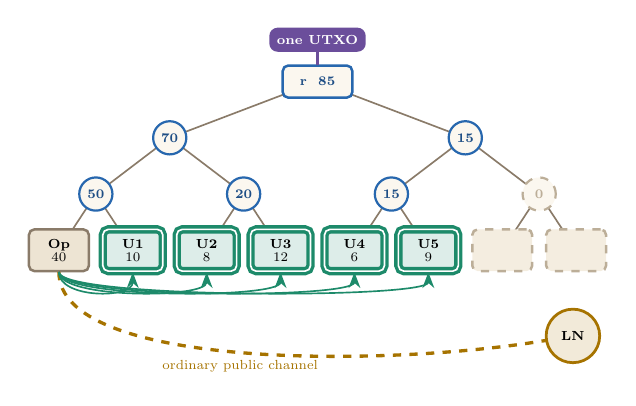
\begin{tikzpicture}[scale=0.68,transform shape,>=Stealth]
        \LTtree[out={one UTXO}]{Op/40/op/, U1/10/chan/, U2/8/chan/, U3/12/chan/, U4/6/chan/, U5/9/chan/, -/0/e/, -/0/e/}
        \node[circle,draw=ltexit,fill=ltexit!15,line width=1pt,font=\scriptsize\bfseries,minimum size=1cm] (pub) at (9.6,-1.6) {LN};
        \draw[ltexit,line width=1.2pt,dashed] (l-0.south) .. controls (0,-2.2) and (6,-2.2) .. (pub) node[pos=0.5,below,font=\scriptsize,text=ltexit] {ordinary public channel};
        \foreach \i in {1,...,5} \draw[ltleaf,line width=0.6pt,->] (l-0.south) .. controls ($(l-0.south)+(0,-0.5)$) and ($(l-\i.south)+(0,-0.5)$) .. (l-\i.south);
      \end{tikzpicture}
    \end{column}
    \begin{column}{0.4\textwidth}
      \small
      A leaf's \code{exit\_key} is the funding output key of a 2-party channel with the operator (MuSig2, LN-Symmetry update machine, Appendix C).
      \begin{itemize}
        \item The funding output doesn't exist yet. It materialises at whatever transition removes the leaf.
        \item Payments between channel leaves are ordinary HTLC forwards through the operator. \hl{Nothing touches the tree}: no spend, no proof, no fee.
        \item Same hash and timelock arithmetic as the public network, so it routes like any LN node.
      \end{itemize}
    \end{column}
  \end{columns}
\end{frame}

\begin{frame}{The price of a channel leaf is patience}
  \begin{itemize}
    \item A force close must first get an \tr{EXIT} confirmed, and that exit competes with every other transition for the single output.
    \item So HTLC deadlines need about \textbf{220 blocks} of \code{cltv\_expiry\_delta} headroom, against 40 to 80 on the public network. The close (exit, update, settlement) takes about \textbf{146 blocks}.
    \item The leaf is \code{SEQ\_FINAL}: not voucher-claimable, and no amount-only top-up without the owner, because its amount is the capacity every signed state commits to.
    \item The lease is the operator's force-close right: \code{evict\_after} is when the operator may put the channel on-chain, and HTLCs must expire before it plus the budget.
    \item \code{chan\_id} binds \code{tree\_id}, so channel states can't be replayed into a sibling tree.
    \item A tower holding an \tr{EXIT}$_K^t$ authorisation and the latest state can \emph{start} the close, not only answer a stale one.
  \end{itemize}
  \lnote{Spec: Appendix C (\texttt{spec/channel-leaves.md}), C.4.4 deadlines, C.6 rules that bind the tree.}
\end{frame}

\begin{frame}{Receiving without a channel: the credit leaf}
  \begin{columns}[T]
    \begin{column}{0.5\textwidth}
      A user with no on-chain funds wants to receive over Lightning.
      \begin{itemize}
        \item The operator funds a \hl{credit leaf} for them.
        \item Each receive: the payer's HTLC reaches the operator, the operator settles it, then signs one cumulative hash-locked voucher for the running total.
        \item Zero on-chain bytes per payment, no minimum, never expires; the recipient can redeem the latest voucher alone.
        \item \tr{CLAIM}$^x$ + \tr{UPDATE}$^x$ + exact payouts: the credit leaf can only grow or pay its recipient.
      \end{itemize}
    \end{column}
    \begin{column}{0.46\textwidth}
      \begin{block}{The gap: it settles first}
        Between settling the HTLC and signing the voucher, the operator holds the payment and the recipient holds nothing enforceable.\\[0.4em]
        Exposure is one payment, but it's trust.\\[0.4em]
        Closing it needs the recipient to hold something \emph{before} releasing the preimage, and the operator to get its money back if the preimage never comes. That's a deadline, which a voucher can't carry.
      \end{block}
    \end{column}
  \end{columns}
\end{frame}

\begin{frame}{Pending pairs: an HTLC that lives in the tree}
  \begin{columns}[c]
    \begin{column}{0.64\textwidth}
      \begin{tikzpicture}[scale=0.84,transform shape]
        \only<1>{\LTtree[region=1/1,regionlabel={receive pair},out={tree output, 23}]{Op/4/op/, Q/3/n/, P/10/pend/until T, L/1/land/, X/5/n/, -/0/e/, -/0/e/, -/0/e/}
          \LTbadge{2}{op owns}{op}\LTbadgeB{2}{R exits}{exit}\LTbadge{3}{R's own}{voucher}}
        \only<2>{\LTtree[region=1/1,regionlabel={receive pair},out={tree output, 23}]{Op/4/op/, Q/3/n/, P/10/pend/until T, L/1/land/, X/5/n/, -/0/e/, -/0/e/, -/0/e/}
          \LTbadge{3}{V$_1$: L$\to$4}{hash}\LTbadgeB{3}{locked to $H_1$}{hash}}
        \only<3>{\LTtree[region=1/1,regionlabel={receive pair},out={tree output, 23}]{Op/4/op/, Q/3/n/, P/10/pend/until T, L/1/land/, X/5/n/, -/0/e/, -/0/e/, -/0/e/}
          \LTbadge{3}{V$_2$: L$\to$6}{hash}\LTbadgeB{3}{locked to $H_2$}{hash}}
        \only<4>{\LTtree[region=1/1,regionlabel={settled},out={tree output, 23}]{Op/4/op/, Q/3/n/, P/5/pend/until T, L/6/new/, X/5/n/, -/0/e/, -/0/e/, -/0/e/}
          \LTbadge{2}{$-5$}{op}\LTbadge{3}{$+5$}{sig}}
        \only<5>{\LTtree[path=2,path2=3,region=1/1,regionlabel={tower redeems V$_2$},out={tree output, 23}]{Op/4/op/, Q/3/n/, P/5/pend/until T, L/6/new/, X/5/n/, -/0/e/, -/0/e/, -/0/e/}
          \LTbadge{3}{V$_2$ + preimage}{hash}}
        \only<6->{\LTtree[path=2,fold=1,rootname={r'},region=1/1,regionlabel={after T: reclaimed},out={tree output, 18}]{Op/4/op/, Q/3/n/, -/0/e/, L/6/n/, X/5/n/, -/0/e/, -/0/e/, -/0/e/}
          \LTbadge{2}{5 back to operator}{op}}
      \end{tikzpicture}
    \end{column}
    \begin{column}{0.34\textwidth}
      \small
      \only<1>{\textbf{P}, pending: owned by the operator, exits to the recipient, evictor \code{RECLAIM\_KEY}, deadline $T$. Funded with the window's expected receipts.\\[0.3em]
        \textbf{L}, landing: the recipient's own leaf, long lease.}
      \only<2>{A payment arrives (hash $H_1$). Before releasing the preimage, the recipient gets a hash-locked \hl{merge voucher}: ``raise P's sibling to 4''.
        Then it reveals the preimage, and the operator settles. \hl{Atomic}: neither side can walk.}
      \only<3>{Another payment: a new voucher to an \emph{absolute} target, $L_0 + \Sigma a_i = 6$.
        Replay is harmless: a target can only be reached once. One voucher per window, however many payments.}
      \only<4>{\textbf{R3, the normal path.} Before $T-\Delta$ the operator's reclaim-form rewrite moves the settled total from P to L, with \emph{only the operator's signature}. Batched across many pairs. \hl{Non-interactive}: the recipient can be asleep.}
      \only<5>{\textbf{R2, if the operator doesn't.} A tower redeems the latest voucher with the preimage (\tr{CLAIM}$^{hm}$: about 1,136 vB in FULL, 626 with the hypothetical opcode). It can only move value \emph{into} a leaf the recipient alone exits, so the tower holds no key.}
      \only<6>{\textbf{R1, after $T$.} The operator reclaims what's left of P with a \code{nLockTime} $\geq T$ (\tr{RECLAIM}$_1$), and must hold the inbound HTLCs until that confirms. Then it rolls a fresh pair.}
    \end{column}
  \end{columns}
\end{frame}

\begin{frame}{R1, R2, R3: three rules, no new opcode}
  \small
  \begin{tabular}{@{}p{1.3cm}p{6.4cm}p{6.3cm}@{}}
    \toprule
    & Rule & Why it's shaped this way \\ \midrule
    \textbf{R1} & A leaf whose evictor is \code{RECLAIM\_KEY} can be removed after its deadline with no payout & the HTLC's timeout branch; a key, not a flag bit, because MID can't isolate a bit \\
    \textbf{R2} & \tr{CLAIM}$^m$: raise the source's \emph{sibling} to an absolute target; target owner $=$ target exit $=$ source exit key & a target the operator could exit or graft could void or drain the voucher; Lean found the exit-key equality was needed \\
    \textbf{R3} & In the reclaim-form rewrite, an even reclaimable leaf may decrease amount-only if its odd sibling rises by exactly the same, with only \code{sig\_op} & batch settlement with nobody online; any other change to a reclaimable leaf takes the R1 branch \\
    \bottomrule
  \end{tabular}
  \vspace{0.3em}

  \begin{columns}[T]
    \begin{column}{0.5\textwidth}
      \begin{tabular}{@{}lr@{}}
        \multicolumn{2}{@{}l}{\textbf{Per pair, per window} (MSU, hypothetical)}\\ \midrule
        no R3: \tr{CLAIM}$^m$ + \tr{RECLAIM}$_1$ & \nPairNoRthree\ vB \\
        R3 batch, 16 positions & \nPairWindowSixteen\ vB \\
        R3 batch, 64 positions & \nPairWindow\ vB \\ \midrule
        \tr{RECLAIM}$_1$ alone, $N{=}2^{16}$ & 490 vB \\
        \tr{CLAIM}$^{hm}$ redeem, $N{=}2^{16}$ & 626 vB \\
      \end{tabular}
    \end{column}
    \begin{column}{0.46\textwidth}
      Per payment: \textbf{zero}. The cost moves to the window, so a merchant with a thousand receives a day pays what a wallet with one does.
      Built end to end in FULL, MID and CCV; MIN can't (no CSFS).
      \muted{These figures assume a proof that can start above height 0; without that, about 480 vB more per merge or rewrite.}
    \end{column}
  \end{columns}
\end{frame}

\begin{frame}{Towers: they choose when, never where}
  \small
  \begin{tabular}{@{}p{4.2cm}p{5.2cm}p{4.4cm}@{}}
    \toprule
    Job & Holds & Deadline it serves \\ \midrule
    keep the path current & leaf, path, the chain & none; everything builds on it \\
    start an exit & an \tr{EXIT}$_K^t$ authorisation, a fee UTXO & the owner's own, or a lease \\
    answer a stale channel state & latest update + settlement & \code{csv\_delay} \\
    redeem a pending-pair voucher & merge voucher, preimage & the pending leaf's $T$ \\
    bump fees, outbid conflicts & a funded UTXO & the contention bound $\Delta(q)$ \\
    \bottomrule
  \end{tabular}
  \vspace{0.8em}
  \begin{itemize}
    \item Every delegable instrument pays a fixed output that belongs to the member. Misuse is bounded to timing: a forced exit of your own funds, paid in full.
    \item Light towers can't watch a fixed scriptPubKey (it changes every transition); they follow the outpoint chain, or ask the operator and check against the confirmed root.
    \item Not designed yet: a tower protocol (registration, payment, hand-off messages).
  \end{itemize}
\end{frame}

% ======================================================================
\section{Opcodes and tiers}

\begin{frame}{No new opcodes: four tiers from existing proposals}
  \small
  \scriptsize
  \begin{tabular}{@{}p{1.0cm}>{\raggedright\arraybackslash}p{6.6cm}>{\raggedright\arraybackslash}p{3.6cm}r@{}}
    \toprule
    Tier & Needs & Carries & Exit, $2^{16}$ \\ \midrule
    \textbf{FULL} & tapleaf \code{0xC2} (BIP-441 restored ops, 64-bit math), \code{OP\_TX}, CSFS (BIP-348), EC ops & everything & 1,020 vB \\
    \textbf{MID} & \code{0xC0}: \code{OP\_CAT}, \code{OP\_TX}, CSFS, \code{OP\_TWEAKADD} (BIP-449) & everything; rewrite $h \leq 5$ & 1,355 vB \\
    \textbf{MIN} & \code{0xC0}: \code{OP\_CAT}, \code{OP\_TWEAKADD}, nothing else & exit and \tr{SPLIT} & 1,473 vB \\
    \textbf{CCV} & \code{OP\_CHECKCONTRACTVERIFY} (BIP-443) + \code{OP\_TX} (+ CSFS for vouchers), either numerics & everything & 908 vB \\
    \midrule
    \muted{floor} & \muted{CCV + a hypothetical \code{OP\_MERKLESUMUPDATE}} & \muted{measurement only} & \muted{about 541 vB} \\
    \bottomrule
  \end{tabular}
  \vspace{0.6em}
  \begin{itemize}
    \item Same tree format in every tier. A rule change lands in every tier that can carry it, or the spec says why not.
    \item MID's 4-byte \code{CScriptNum}: leaves arrive as fields, amounts as numbers plus \code{PADZ} pads.
    \item Liquid has most of MID today: the obvious place for a prototype.
  \end{itemize}
\end{frame}

\begin{frame}{MIN: introspection recovered from \texttt{OP\_CHECKSIG}}
  \begin{columns}[T]
    \begin{column}{0.55\textwidth}
      MIN has no introspection opcode, but \code{OP\_CHECKSIG} \emph{does} see the transaction.
      \begin{enumerate}
        \item The script builds the BIP-341 signature message itself from the values it wants to constrain (outputs, amounts) with \code{OP\_CAT}.
        \item It hashes it and computes the signature for key $G$ and nonce $G$: $s = 1 + e$, a value the script can derive (\code{OP\_TWEAKADD}).
        \item \code{OP\_CHECKSIG} hashes the \emph{real} transaction. It passes only if the constructed message equals the real one.
      \end{enumerate}
    \end{column}
    \begin{column}{0.41\textwidth}
      \begin{block}{What it shows}
        The signature authorises nothing; it \hl{binds}. Every field the script pinned is enforced.\\[0.4em]
        The load-bearing operation, a one-transaction exit, needs only \code{OP\_CAT} and one point-tweak opcode.\\[0.4em]
        It's an upper bound on what's required, not a recommendation: 43\% more than FULL, and only exit and \tr{SPLIT}.
      \end{block}
    \end{column}
  \end{columns}
\end{frame}

\begin{frame}{The floor: one Merkle-sum opcode}
  \begin{columns}[T]
    \begin{column}{0.52\textwidth}
      Unrolling the fold is most of the script. A single opcode that verifies a Merkle-sum path and returns the updated root replaces the fold and the sum arithmetic along the path. Then:
      \begin{itemize}
        \item the exit script is \textbf{252 bytes at any depth}, dense or sparse,
        \item the proof is one 40-byte sibling per \emph{occupied} level,
        \item a key-addressed tree of depth 64 is practical,
        \item an exit is \textbf{about 381 + 10$\log_2 N$ vB}.
      \end{itemize}
      The scripts still do arithmetic for pending receives and lock-time checks.
    \end{column}
    \begin{column}{0.44\textwidth}
      \begin{block}{Status}
        Specified and measured in the simulator behind a \code{hypothetical} flag (\nChecksMSU\ checks).
        Quarantined from every tier and golden vector.
        Nobody has proposed it for Bitcoin.\\[0.4em]
        Later slides mark the figures that use it (541, 626, 547 vB). The rest are FULL or the named tier.\\[0.4em]
        626 and 547 also assume a proof that can start above height 0; without that, about 480 vB more per merge or rewrite.
      \end{block}
    \end{column}
  \end{columns}
\end{frame}

% ======================================================================
\section{Performance and scalability}

\begin{frame}{Leaving alone: 10 vB per doubling}
  \begin{columns}[c]
    \begin{column}{0.62\textwidth}
      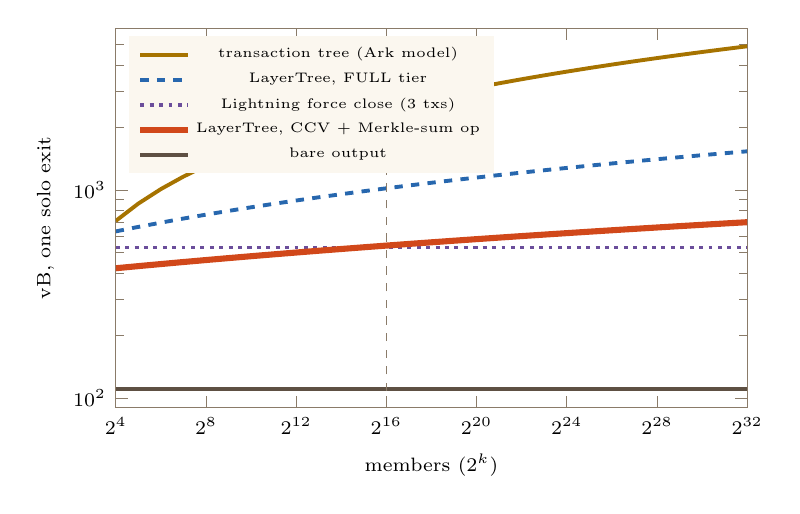
\begin{tikzpicture}
        \begin{axis}[width=9.6cm,height=6.4cm,ymode=log,xmin=4,xmax=32,ymin=90,ymax=6000,
            xlabel={members ($2^k$)},ylabel={vB, one solo exit},
            xtick={4,8,12,16,20,24,28,32},xticklabels={$2^4$,$2^8$,$2^{12}$,$2^{16}$,$2^{20}$,$2^{24}$,$2^{28}$,$2^{32}$},
            log basis y=10,yticklabel style={font=\scriptsize},xticklabel style={font=\scriptsize},
            label style={font=\scriptsize},axis line style={ltstrong},tick style={ltstrong},
            legend style={font=\tiny,draw=none,fill=ltsurface,at={(0.02,0.98)},anchor=north west},
            every axis plot/.append style={line width=1.4pt},samples=29,domain=4:32]
          \addplot[ltexit] {150*x+111}; \addlegendentry{transaction tree (Ark model)}
          \addplot[ltnode,dashed] {504+32.25*x}; \addlegendentry{LayerTree, FULL tier}
          \addplot[ltchain,dotted] {530}; \addlegendentry{Lightning force close (3 txs)}
          \addplot[ltaccent,line width=2.2pt] {381+10*x}; \addlegendentry{LayerTree, CCV + Merkle-sum op}
          \addplot[ltmuted] {111}; \addlegendentry{bare output}
          \draw[ltstrong,dashed,line width=0.5pt] (axis cs:16,90) -- (axis cs:16,6000);
        \end{axis}
      \end{tikzpicture}
    \end{column}
    \begin{column}{0.36\textwidth}
      \small
      \begin{tabular}{@{}lrrr@{}}
        \toprule
        members & LT & FULL & tree \\ \midrule
        $2^{8}$ & 461 & 762 & 1,311 \\
        $2^{16}$ & 541 & 1,020 & 2,511 \\
        $2^{20}$ & 581 & 1,149 & 3,111 \\
        $2^{32}$ & 701 & 1,536 & 4,911 \\
        \bottomrule
      \end{tabular}\\[0.6em]
      LT is CCV with the hypothetical opcode: $381 + 10\log_2 N$ vB, one 40-byte sibling per occupied level.
      A transaction tree pays a whole $\sim$150 vB transaction per level.\\[0.4em]
      \muted{At $2^{16}$: 4.6$\times$ smaller; at $2^{32}$: 7$\times$.}
    \end{column}
  \end{columns}
\end{frame}

\begin{frame}{One transaction is the safety property}
  \begin{columns}[c]
    \begin{column}{0.5\textwidth}
      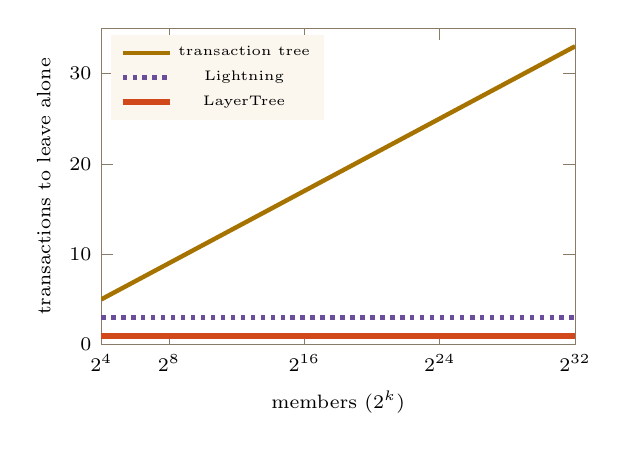
\begin{tikzpicture}
        \begin{axis}[width=7.6cm,height=5.6cm,xmin=4,xmax=32,ymin=0,ymax=35,
            xlabel={members ($2^k$)},ylabel={transactions to leave alone},
            xtick={4,8,16,24,32},xticklabels={$2^4$,$2^8$,$2^{16}$,$2^{24}$,$2^{32}$},
            yticklabel style={font=\scriptsize},xticklabel style={font=\scriptsize},label style={font=\scriptsize},
            axis line style={ltstrong},tick style={ltstrong},
            legend style={font=\tiny,draw=none,fill=ltsurface,at={(0.02,0.98)},anchor=north west},
            every axis plot/.append style={line width=1.6pt},samples=29,domain=4:32]
          \addplot[ltexit] {x+1}; \addlegendentry{transaction tree}
          \addplot[ltchain,dotted] {3}; \addlegendentry{Lightning}
          \addplot[ltaccent,line width=2.2pt] {1}; \addlegendentry{LayerTree}
        \end{axis}
      \end{tikzpicture}
    \end{column}
    \begin{column}{0.48\textwidth}
      \small
      \scriptsize
      \begin{tabular}{@{}>{\raggedright\arraybackslash}p{1.7cm}>{\raggedright\arraybackslash}p{1.2cm}>{\raggedright\arraybackslash}p{1.1cm}>{\raggedright\arraybackslash}p{1.5cm}@{}}
        \toprule
        at $2^{16}$ & LayerTree & LN close & tx tree \\ \midrule
        transactions & 1 & 3 & 17 \\
        blocks to spend & 1 & $\sim$145 & 16 + leaf lock \\
        who must be online & nobody & a tower & you, before expiry \\
        what expires & nothing & nothing & the round \\
        \bottomrule
      \end{tabular}\\[0.8em]
      Each extra transaction is another fee at that day's rate, and another place a low-fee ancestor or a conflicting spend can hold you up. Under fee pressure, or in a mass exit, or with a hostile operator, \hl{one transaction beats seventeen}.
    \end{column}
  \end{columns}
\end{frame}

\begin{frame}{Batching: the per-leaf cost falls with the batch}
  \begin{columns}[c]
    \begin{column}{0.62\textwidth}
      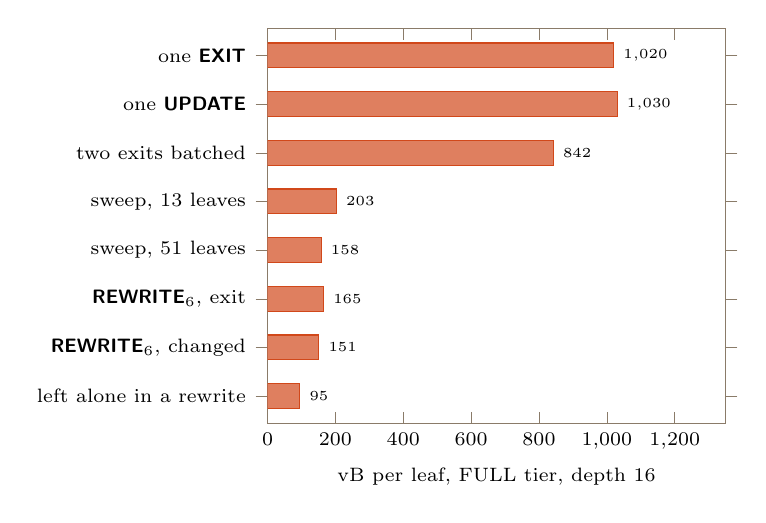
\begin{tikzpicture}
        \begin{axis}[xbar,width=7.4cm,height=6.6cm,xmin=0,xmax=1350,
            symbolic y coords={unch,rwup,rwex,sw51,sw13,ex2,up1,ex1},ytick=data,
            yticklabels={{left alone in a rewrite},{\tr{REWRITE}$_6$, changed},{\tr{REWRITE}$_6$, exit},{sweep, 51 leaves},{sweep, 13 leaves},{two exits batched},{one \tr{UPDATE}},{one \tr{EXIT}}},
            yticklabel style={font=\scriptsize},xticklabel style={font=\scriptsize},
            xlabel={vB per leaf, FULL tier, depth 16},label style={font=\scriptsize},
            axis line style={ltstrong},tick style={ltstrong},bar width=9pt,
            nodes near coords,nodes near coords style={font=\tiny},enlarge y limits=0.08]
          \addplot[fill=ltaccent!70,draw=ltaccent] coordinates {(95,unch) (151,rwup) (165,rwex) (158,sw51) (203,sw13) (842,ex2) (1030,up1) (1020,ex1)};
        \end{axis}
      \end{tikzpicture}
    \end{column}
    \begin{column}{0.36\textwidth}
      \footnotesize
      Owners exiting together each carry a full path, so a pair saves only the fixed overhead.\\[0.4em]
      A cohort shares one path above its subtree: the sweep (operator, after a lease) and the rewrite (owners, any time) hash the interior once.\\[0.4em]
      \hl{Tapscript has no loops}: the per-position step is published in every batch. That script is most of a batch's cost, and the reason the next ideas focus on batches.\\[0.3em]\msuTBD{batching-chart}
    \end{column}
  \end{columns}
\end{frame}

\begin{frame}{Per member, over a lifetime}
  \small
  \centering
  \begin{tabular}{@{}lrrr@{}}
    \toprule
    vB per member, entering in a batch & never exits alone & exits in a batch & exits alone \\ \midrule
    \textbf{LayerTree, CCV + Merkle-sum op} & \textbf{3} & \textbf{161} & \textbf{544} \\
    LayerTree, FULL tier & 3 & 161 & 1,023 \\
    Lightning channel & 197 & 197 & 573 \\
    Transaction tree (Ark model) & 86 & 86 & 2,554 \\
    Bare output & 154 & 154 & 154 \\
    \bottomrule
  \end{tabular}
  \vspace{1em}
  \begin{itemize}
    \item Entry is nearly free: a cohort graft of 1,024 members is 614 vB (FULL), \textbf{under 1 vB each}, when the operator funds it and members buy balances off-chain.
    \item A member who's swept at lease end, or sells their balance by voucher, pays almost nothing.
    \item A member who exits alone pays for the proof, and loses to a bare UTXO and roughly ties Lightning.
    \item The UTXO set: a tree of any size is \hl{one output}.
  \end{itemize}
\end{frame}

\begin{frame}{When everyone leaves at once}
  \small
  \centering
  \begin{tabular}{@{}rrrrrr@{}}
    \toprule
    members & one tree & sharded ($2^{10}$) & sharded, cohort exits & tx tree & Lightning \\ \midrule
    1,024 & 41 & 41 & 11 & 1 & 1 \\
    65,536 & 2,622 & 41 & 11 & 18 & 35 \\
    1,048,576 & 41,944 & 610 & 173 & 274 & 556 \\
    \bottomrule
  \end{tabular}\\[0.3em]
  {\scriptsize\muted{Blocks until every member has left, nobody cooperating; 1 MvB per block; 25 exits per tree per block; cohort exits remove 64 members per transaction at about 165 vB each (FULL).}}
  \vspace{0.8em}
  \begin{itemize}
    \item Every exit spends the same output, so one tree's exits queue: about 25 per block under the descendant limit, up to 64 under cluster mempool.
    \item One tree of 65,536 drained one stranger at a time takes about 18 days. So: \hl{size each tree by exit throughput}, shard deployments, and \tr{DETACH} a cohort on demand.
    \item Sharded with cohort exits, LayerTree drains faster than any design in the table. At a million members everyone is block-space bound and the cheaper exit wins.
  \end{itemize}
\end{frame}

% ======================================================================
\section{Trade-offs}

\begin{frame}{Where it loses}
  \begin{itemize}
    \item \textbf{Against a bare output, on every solo exit.} 541 vB with the hypothetical opcode (1,020 in FULL) against 111. The proof is the price of sharing, and only batching gets it back.
    \item \textbf{Level with a Lightning force close in bytes only with the hypothetical opcode} (541 against 530 vB; FULL is about twice), but one transaction and one block against three and about a day.
    \item \textbf{A non-cooperative mass exit from one big tree.} Exits serialise through one output; transaction-tree branches unroll in parallel.
    \item \textbf{On-chain payments.} An \tr{UPDATE} is about 1,030 vB (FULL; \msuTBD{update}). Value has to move off-chain: channel leaves, vouchers, or batched rewrites.
    \item \textbf{It needs opcodes that aren't active.} With today's proposals the cheapest exit is CCV's 908 vB; the 541 vB figures assume an opcode nobody has proposed.
    \item \textbf{Joining needs the operator.} No liveness guarantee for getting in, only for getting out.
  \end{itemize}
\end{frame}

\begin{frame}{One output, one queue}
  \begin{columns}[T]
    \begin{column}{0.54\textwidth}
      Every transition spends and recreates the same UTXO, so unconfirmed transitions form a chain.
      \begin{itemize}
        \item An honest exit can be displaced by any conflicting spend that confirms first, and must be rebuilt against the new root.
        \item The spec doesn't pretend to derive liveness: assumption \textbf{[C]} names it. At most $\beta$ conflicting spends ahead, $\kappa$ per block, so an exit lands within
          $\Delta(q) = \Delta_L(\lceil(\beta+q)/\kappa\rceil + 1)$.
        \item Fee pinning is outside [C]: one cheap transition early in the queue caps the fee rate of everything behind it.
      \end{itemize}
    \end{column}
    \begin{column}{0.42\textwidth}
      \begin{block}{The structural answers}
        \begin{itemize}
          \item shard: many trees, each sized by exit throughput
          \item \tr{DETACH}$_h$: a cohort gets its own output and its own chain
          \item batches count once against the limit
          \item \tr{EXIT}$_K^t$: a tower rebuilds and rebroadcasts with the owner offline
          \item cluster mempool raises $\kappa$ for a cooperative tree
        \end{itemize}
      \end{block}
      \muted{\small This is the design's real weak spot.}
    \end{column}
  \end{columns}
\end{frame}

\begin{frame}{The trust model}
  \begin{columns}[T]
    \begin{column}{0.48\textwidth}
      \begin{block}{The operator can}
        \begin{itemize}
          \item add members (graft into empty slots)
          \item co-sign cooperative changes
          \item top up a leaf (amount only)
          \item evict a leaf after its lease, paying it in full
          \item reclaim a pending leaf after its deadline
          \item refuse to let you in, and grief cheaply
        \end{itemize}
      \end{block}
    \end{column}
    \begin{column}{0.48\textwidth}
      \begin{block}{The operator cannot}
        \begin{itemize}
          \item take a satoshi of anyone's leaf
          \item stop you leaving, or delay you past [C]
          \item change your keys or shorten your lease
          \item replay a voucher, or void one you hold in a pending pair before its deadline
        \end{itemize}
      \end{block}
    \end{column}
  \end{columns}
  \vspace{0.6em}
  \textbf{What members must do:} keep their own path data (proofs are data availability), check their path inside a cohort \emph{before} funding a graft (a fake subtree freezes value, it can't create it), and watch leases and deadlines, or hand that to a tower.
\end{frame}

% ======================================================================
\section{How we know it's right}

\begin{frame}{Rules proved, scripts executed, two implementations agreeing}
  \small
  \begin{tabular}{@{}p{3.4cm}p{10.4cm}@{}}
    \toprule
    Layer & Checked by \\ \midrule
    the rules (spec 7) & Lean 4, \textbf{\nLean\ theorems}, no Mathlib, no \code{sorry}, axiom-audited \\
    the scripts & a tapscript simulator with the real BIP-341 sighash: \nChecksFULL\ FULL, \nChecksMID\ MID, \nChecksMIN\ MIN, \nChecksCCV\ CCV, \nChecksCHAN\ channel-leaf checks, positive and negative per rule \\
    Python against Go & byte-exact golden scripts and a shared sighash vector \\
    Go-built witnesses & \nReplay\ end-to-end transactions from the Go builders, replayed through the simulator \\
    composition & a UC argument with the Lean theorems as extraction lemmas (the paper) \\
    \bottomrule
  \end{tabular}
  \vspace{0.6em}
  \begin{itemize}
    \item Conservation holds for every valid sequence of steps, \hl{unconditionally}. Payability (any holder can build an accepted exit) needs the real-tree invariant, which grafting must establish off-chain: the proofs forced that distinction into the open.
    \item The proofs changed the design: the merge claim's target needs \code{exit\_key} equality, or a cycle of merges and a different-key target were possible.
    \item Not covered: the link from rules to bytecode is execution, not proof. A P model of the off-chain protocol is designed, not built.
  \end{itemize}
\end{frame}

% ======================================================================
\section{Future directions}

\begin{frame}{Optimistic batches: publish the root, not the leaves}
  \muted{\small A sketch for discussion: not in the spec, not reviewed.}\\[0.4em]
  \begin{columns}[T]
    \begin{column}{0.5\textwidth}
      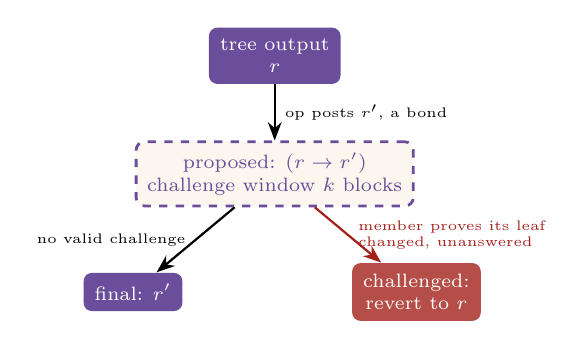
\begin{tikzpicture}[>=Stealth,b/.style={rectangle,rounded corners=3pt,font=\scriptsize,align=center,inner sep=4pt}]
        \node[b,fill=ltchain,text=white] (a) at (0,3) {tree output\\$r$};
        \node[b,draw=ltchain,dashed,line width=1pt,fill=ltsurface,text=ltchain] (p) at (0,1.5) {proposed: $(r \to r')$\\challenge window $k$ blocks};
        \node[b,fill=ltchain,text=white] (f) at (-1.8,0) {final: $r'$};
        \node[b,fill=ltbad!80,text=white] (c) at (1.8,0) {challenged:\\revert to $r$};
        \draw[->,thick] (a) -- node[right,font=\tiny]{op posts $r'$, a bond} (p);
        \draw[->,thick] (p) -- node[left,font=\tiny]{no valid challenge} (f);
        \draw[->,thick,ltbad] (p) -- node[right,font=\tiny,align=left]{member proves its leaf\\changed, unanswered} (c);
      \end{tikzpicture}
    \end{column}
    \begin{column}{0.48\textwidth}
      \small
      Today a rewrite publishes every slot twice and verifies everything: about 151 vB per changed leaf.\\[0.4em]
      Optimistically, the operator publishes only the new root (and a commitment to the change set). For $k$ blocks:
      \begin{itemize}
        \item a member proves its leaf under $r$ and its slot under $r'$ differ, or asks for its new path;
        \item the operator answers with the member's signature over the change, or the path, on-chain;
        \item no answer: the proposal reverts and the bond pays the challenger.
      \end{itemize}
      Happy path: a constant-size transaction, whatever the batch.
    \end{column}
  \end{columns}
\end{frame}

\begin{frame}{What the optimistic version trades}
  \begin{columns}[T]
    \begin{column}{0.48\textwidth}
      \begin{block}{Gains}
        \begin{itemize}
          \item batch cost independent of batch size: per-leaf cost toward zero
          \item fewer bytes than even a native Merkle-sum opcode's batch
          \item the existing exit stays the escape hatch: nobody's exit gets worse
        \end{itemize}
      \end{block}
    \end{column}
    \begin{column}{0.48\textwidth}
      \begin{block}{Costs and open questions}
        \begin{itemize}
          \item liveness: someone must watch every window (towers)
          \item data availability: withheld paths become on-chain challenges
          \item latency: a batch is final only after $k$ blocks, and the output carries two roots meanwhile
          \item griefing: bond sizing for both sides
          \item exits in the window must hold under both roots
          \item needs CSFS and two-root state (CCV fits)
        \end{itemize}
      \end{block}
    \end{column}
  \end{columns}
  \lnote{Today's design is the pessimistic end: every batch carries its own proof, so no window and no watchers.}
\end{frame}

\begin{frame}{Other directions}
  \begin{columns}[T]
    \begin{column}{0.5\textwidth}
      \begin{itemize}
        \item \textbf{Cheaper rewrite steps.} Just landed: an 8-byte amount-only element in place of a republished 116-byte leaf (587 $\to$ 547 vB per settled pair, with the hypothetical opcode). The per-position script is now most of a batch's cost.
        \item \textbf{A native Merkle-sum opcode.} 252 bytes of script at any depth; key-addressed trees of depth 64. It helps exits, not batches. Worth proposing?
        \item \textbf{Liquid prototype of MID.} Most of the opcodes exist there today.
        \item \textbf{Signet / Inquisition harness} to confirm the throughput and TRUC-anchor assumptions on a real node.
      \end{itemize}
    \end{column}
    \begin{column}{0.48\textwidth}
      \begin{itemize}
        \item \textbf{The P model} of the off-chain protocol: covenant oracle, watchtower with lag, adversarial timing.
        \item \textbf{A verified compiler} from rules to tapscript, closing the gap the simulator covers today.
        \item \textbf{PTLCs and second-stage HTLCs} for channel leaves.
        \item \textbf{A tower protocol}: registration, payment, hand-off of authorisations and vouchers.
        \item \textbf{Cross-tree swaps} and splicing between shards.
      \end{itemize}
    \end{column}
  \end{columns}
\end{frame}

\begin{frame}[plain]
  \centering
  \vfill
  {\color{ltaccent}\rule{2cm}{2pt}}\\[0.6em]
  {\Huge\bfseries Questions}\\[1em]
  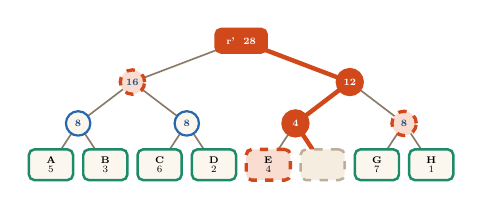
\begin{tikzpicture}[scale=0.5,transform shape]
    \LTtree[path=5,fold=1,rootname={r'}]{A/5/n/, B/3/n/, C/6/n/, D/2/n/, E/4/n/, -/0/e/, G/7/n/, H/1/n/}
  \end{tikzpicture}
  \vfill
\end{frame}

% ======================================================================
\appendix
\section{Backup}

\begin{frame}{Backup: one level of the fold, old and new together}
  \scriptsize\let\code\codes
  \begin{columns}[T]
    \begin{column}{0.62\textwidth}
      Before: \code{dir sc T oh os nh ns}. Names are without \code{OP\_}; the sequence is spec 8.2 \code{LEVEL} (88 B).
      \setlength{\tabcolsep}{3pt}
      \begin{tabular}{@{}p{4.3cm}p{3.9cm}@{}}
        \toprule
        opcodes & stack (altstack after $|$) \\ \midrule
        \code{6 ROLL 6 ROLL} & \code{T oh os nh ns dir sc} \\
        \code{SIZE 41 EQUALVERIFY DUP 32 8 SUBSTR DUP TOALTSTACK} & \code{\ldots\ dir sc ss8} $|$ \code{ss8} \\
        \multicolumn{2}{@{}l}{\hl{new half}}\\
        \code{3 ROLL TUCK ADD TOALTSTACK PAD8} & \code{T oh os nh dir sc ns9} $|$ \code{ss8 ns'} \\
        \code{3 ROLL SWAP CAT} & \code{T oh os dir sc nc}, \code{nc = nh||enc64(ns)} \\
        \code{OVER SWAP 3 PICK NOTIF SWAP ENDIF CAT} & \code{\ldots\ dir sc pre\_n}: \code{dir ? sc||nc : nc||sc} \\
        \code{5 PICK SWAP CAT SHA256 TOALTSTACK} & \code{T oh os dir sc} $|$ \code{ss8 ns' nh'} \\
        \code{FROMALTSTACK} $\times3$ & \code{T oh os dir sc nh' ns' ss8} \\
        \multicolumn{2}{@{}l}{\hl{old half}, same siblings}\\
        \code{5 ROLL TUCK ADD TOALTSTACK PAD8}, \code{5 ROLL SWAP CAT} & \code{T dir sc nh' ns' oc}, \code{oc = oh||enc64(os)} \\
        \code{3 ROLL SWAP 4 ROLL NOTIF SWAP ENDIF CAT}, \code{3 PICK SWAP CAT SHA256}, \code{FROMALTSTACK 2SWAP} & \code{T oh' os' nh' ns'} \\
        \bottomrule
      \end{tabular}
    \end{column}
    \begin{column}{0.35\textwidth}
      \centering
      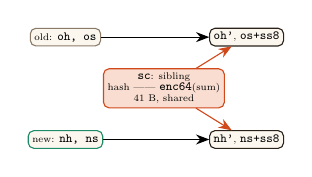
\begin{tikzpicture}[scale=0.5,transform shape,b/.style={rectangle,rounded corners=2pt,draw=ltink,fill=ltsurface,font=\scriptsize,align=center,inner sep=3pt},>=Stealth]
        \node[b,draw=ltstrong] (o) at (0,2.6) {old: \code{oh, os}};
        \node[b,draw=ltleaf] (n) at (0,0) {new: \code{nh, ns}};
        \node[b,draw=ltaccent,fill=ltaccentsoft] (s) at (2.5,1.3) {\code{sc}: sibling\\hash || \code{enc64}(sum)\\41 B, shared};
        \node[b] (po) at (4.6,2.6) {\code{oh'}, \code{os+ss8}};
        \node[b] (pn) at (4.6,0) {\code{nh'}, \code{ns+ss8}};
        \draw[->] (o) -- (po); \draw[->] (n) -- (pn);
        \draw[->,ltaccent] (s) -- (po); \draw[->,ltaccent] (s) -- (pn);
      \end{tikzpicture}\\[0.4em]
      \raggedright
      \code{dir} (empty or \code{0x01}) says which side \code{sc} goes on, for both hashes.\\[0.3em]
      \code{ss8} (low 8 bytes of the sibling's sum) is added to both sums, so the totals differ only by the leaf. Witness per level: \code{sc} 41 B plus \code{dir} 0 or 1 B.
    \end{column}
  \end{columns}
\end{frame}

\begin{frame}{Backup: the post-order rewrite machine, $h = 2$}
  \scriptsize\let\code\codes
  \begin{columns}[T]
    \begin{column}{0.46\textwidth}
      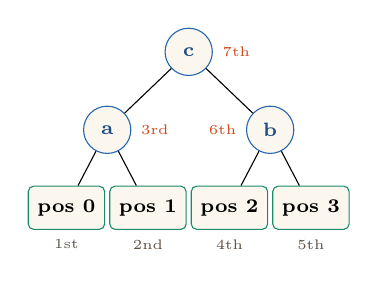
\begin{tikzpicture}[scale=0.9,
          p/.style={rectangle,rounded corners=2pt,draw=ltleaf,fill=ltsurface,minimum width=0.9cm,minimum height=0.55cm,font=\scriptsize\bfseries},
          h/.style={circle,draw=ltnode,fill=ltsurface,minimum size=0.6cm,inner sep=0pt,font=\scriptsize\bfseries,text=ltnodesum},>=Stealth]
        \foreach \i in {0,1,2,3} \node[p] (p\i) at (\i*1.15,0) {pos \i};
        \node[h] (a) at (0.575,1.1) {a}; \node[h] (b) at (2.875,1.1) {b}; \node[h] (c) at (1.725,2.2) {c};
        \draw (p0)--(a) (p1)--(a) (p2)--(b) (p3)--(b) (a)--(c) (b)--(c);
        \node[font=\tiny,text=ltmuted,anchor=north] at (p0.south) {1st};
        \node[font=\tiny,text=ltmuted,anchor=north] at (p1.south) {2nd};
        \node[font=\tiny,text=ltmuted,anchor=north] at (p2.south) {4th};
        \node[font=\tiny,text=ltmuted,anchor=north] at (p3.south) {5th};
        \node[font=\tiny,text=ltaccent,right] at (a.east) {3rd};
        \node[font=\tiny,text=ltaccent,left] at (b.west) {6th};
        \node[font=\tiny,text=ltaccent,right] at (c.east) {7th};
      \end{tikzpicture}\\[0.5em]
      Each position yields four items \code{oh os nh ns}. A \code{HASH\_STEP2} runs as soon as two siblings are on top: the old pair first, then the new pair. The running sum of a hash waits on the altstack; the next output index \code{idx} sits there under the whole machine ($|$ \code{m r idx}).
    \end{column}
    \begin{column}{0.52\textwidth}
      \code{REWRITE\_2}, spec 8.9 and \code{structured/REWRITE\_2\_D8.txt}; $d$ is the number of machine items above \code{T}.\\[0.3em]
      \setlength{\tabcolsep}{3pt}
      \begin{tabular}{@{}lll@{}}
        \toprule
        step & argument $d$ & $d$ after \\ \midrule
        push \code{Z L T} & & 0 \\
        \code{REWRITE\_STEP} & 0 & 4 \\
        \code{REWRITE\_STEP} & 4 & 8 \\
        \code{HASH\_STEP2} & 8 & 4 \\
        \code{REWRITE\_STEP} & 4 & 8 \\
        \code{REWRITE\_STEP} & 8 & 12 \\
        \code{HASH\_STEP2} & 12 & 8 \\
        \code{HASH\_STEP2} & 8 & 4 \\
        \bottomrule
      \end{tabular}\\[0.4em]
      Only $d$-dependent: the roll of the next witness slot (\code{d+3}, \code{d+4}), the picks of \code{T}, \code{L}, \code{Z}. \code{HASH\_STEP2} moves its eight items with constants:\\[0.2em]
      \code{2SWAP 7 ROLL 7 ROLL 2SWAP HASH\_STEP(d)}\\
      \code{2SWAP 5 ROLL 5 ROLL 2SWAP HASH\_STEP(d-2)}\\[0.4em]
      \code{d = 12} first appears at $h = 2$, so test a new shape there, not at $h = 1$. After the machine, \code{LEVEL} $\times (D-h)$ folds the one path above.
    \end{column}
  \end{columns}
\end{frame}

\end{document}
